% main.tex

\documentclass[10pt, titlepage, a4paper]{article}

% Packages 
\usepackage{graphicx}
\usepackage[export]{adjustbox}
\usepackage{amsmath}
\usepackage{amsfonts}
\usepackage{fancyhdr}
\usepackage{enumerate}
\usepackage{listings}
\usepackage[titletoc,toc]{appendix}
\usepackage[pdfborder={0 0 0},colorlinks=true, urlcolor=blue, citecolor=red, bookmarks=false]{hyperref}
\usepackage[margin=3cm]{geometry}
\usepackage[absolute]{textpos}
\usepackage[section]{placeins}
\usepackage{url}
\usepackage{tabularx}
% \usepackage{gensymb}
\usepackage{caption}
% \usepackage{xltxtra}


% for citations
\usepackage{dirtytalk}

%For Swedish
\usepackage[utf8]{inputenc}

%For a table /Falk
\usepackage{graphicx}

%fiddling around with quotes
\usepackage{csquotes}
\usepackage{blindtext} % REMOVE LATER

%fiddling with rotation
\usepackage{adjustbox}

% Page style
\pagestyle{fancy}
\marginparsep = 0pt

% Set font
% \setromanfont{Calibri}

\renewcommand\contentsname{Table of Contents}
\newcommand{\HRule}{\rule{\linewidth}{0.5mm}}
	
\newcommand{\circR}{\textsuperscript{\textregistered}}

% Code style
\lstset{
	backgroundcolor=\color[rgb]{0.92,0.92,0.92},
	basicstyle=\footnotesize,
	showspaces=false,
	showstringspaces=false,
	showtabs=false,
	tabsize=2,
	captionpos=b,
	breaklines=false,
	keywordstyle=\color[rgb]{0,0,1},
	commentstyle=\color[rgb]{0.133,0.545,0.133}
}

\begin{document}
    \begin{titlepage}
        % Title
        % title.tex	

\begin{center}

	\begin{figure}[t]	
		\includegraphics[width=25mm]{MDHlogga.png}
	\end{figure}
    \Large M\"{a}lardalen University \\
    \Large School of Innovation, Design and Engineering \\
    \Large V\"{a}ster\r{a}s, Sweden\\

    \noindent\makebox[\linewidth]{\rule{\textwidth}{0.4pt}}\\
    [0.5cm]
                
    \Large{Project Course in Robotics and Embedded Systems,\\
    CDT508 and DVA425}\\
    [2.0cm]

	\huge \textbf{\uppercase{The Butler Project}} \\ 
    [1.85cm] 
				
    \begin{tabular}{@{}ll}
    
		\Large Examiner: & 
		\begin{minipage}[t]{0,7\textwidth}
		    \Large Mikael Ekstr\"om\\
		    \large M\"{a}lardalen University, 
		    \large V\"{a}ster\r{a}s, Sweden\\ 
		\end{minipage}\\
		[0.5cm]
			
		\Large Project Manager: & 
		\begin{minipage}[t]{0,7\textwidth}
		    \Large Henrik Falk\\
		    \large M\"{a}lardalen University, 
		    \large V\"{a}ster\r{a}s, Sweden 
		\end{minipage}\\
		[0.5cm]
		
	    \Large Editors: &
	    \begin{minipage}[t]{0,7\textwidth}
	    \Large Niclas Holmqvist \\
	    \Large Armantal Hasanbegovic \\
	    \Large Martin Johansson\\
	    \Large Anders Persson\\
	    \large M\"{a}lardalen University,
	    \large V\"{a}ster\r{a}s, Sweden
	    \end{minipage}\\
	    \\
		\Large Research Partners: & 
		\begin{minipage}[t]{0,7\textwidth}
            % \large Mälardalen University\\
            % \large Volvo CE\\
            % \large Husqvarna\\
            % \vspace{0.01ex}
            \includegraphics[width=25mm, valign=t]{images/mdh.png}
		    \includegraphics[width=25mm, valign=t]{images/dpac.png}
		    \includegraphics[width=25mm, valign=t]{images/volvo.png}
		    \includegraphics[width=25mm, valign=t]{images/husqvarna.png}
        \end{minipage}\\
        \\
        \vspace{1.5ex}
        \Large Sponsors: & 
        \begin{minipage}[t]{0,7\textwidth}
            % \large Aratron\\
            % \large Rollco\\
            % \large W\"urth Electronics\\
            % \large Avans\\
            % \large Mekanex\\
            % \vspace{0.000001ex}
            \hspace{-0.5em}
		    \includegraphics[width=25mm, valign=t]{images/aratron.png}
		    \includegraphics[width=25mm, valign=t]{images/rollco.png}
		    \includegraphics[width=25mm, valign=t]{images/wurth.png}
            \includegraphics[width=25mm, valign=t]{images/avans.png}
        
        \end{minipage}
    
    \end{tabular}
    
    \vspace*{\fill}
    \large \today
    
\end{center}


    \end{titlepage}

    % Page style
    \thispagestyle{fancy}
    \fancyhead[R]{The Butler Project}
    \fancyhead[L]{M\"{a}lardalen University}
    \renewcommand{\headrulewidth}{0.4pt}
    \renewcommand{\footrulewidth}{0.4pt}

    % Begin actual text

    % \def\abstract{
    %     \vfil
    %     \begin{center}
    %         {\bfseries\abstractname\vspace{-.5em}}
    %     \end{center}
    %     \itshape
    %     }
    % \def\endabstract{\par}

    % % ============================= Abstract ==============================
    % \begin{abstract}
To be written
\end{abstract}
    % \newpage
    
    \section*{Acknowledgements}
\noindent Our big thanks goes out to our supervisor and examiner, Mikael Ekström. He has supported us throughout the project with his presence and absence.\\ 

\noindent Bengt-Erik Gustavsson and the workshop crew (Axel Öberg, Henrik Lekryd, Barret Sauter) at Mälardalen University Eskilstuna, for providing invaluable assistance and feedback in design and manufacturing. \\

\noindent We could not have come as far as we did without our sponsors, Aratron, Rollco, W\"{u}rth Electronics and, Avans. A big thank you. \\

\noindent We would also like to thank previous members of the Butler Project, Jakob Danielsson, Daniel Jonasson, Rickard Holm and, Roxanne Anderberg. Their insight and knowledge of the Butler helped us find our way.\\

\noindent A thank you to Husqvarna with representatives Peter Jägenstedt, Björn Mannefred and Stefan Grufman. Their research platform is a step towards the future.\\

\noindent Throughout the project we have received fresh batches of cookies for consumption by the team. Thank you Elsy Falk, mother of Henrik Falk, for brightening up our environment.\\
    \newpage

    % ======================= Table of contents ===========================
    \hypersetup{linkcolor=black}
    \tableofcontents
    \hypersetup{linkcolor=red}
    \newpage

    % ============================== Content ==============================
    
    \section{Project Description - Henrik Falk}
MDH@HOME with the robot named Butler is a project realised by students at Mälardalen University. The project aims to build a Human Services Robot (HSR) together with Volvo CE in Eskilstuna. It is a project that spans over 5 years with the end goal of running a robot café autonomously. This report presents the development for the project's third year.

\subsection{Background}
The project was initialised during the fall of 2015 with a the aim of creating a HSR that would be able to compete in RoboCup@HOME. At the start of this project there existed a \say{go and grasp}-task within the competition. The MDH@HOME Butler aims to be the quickest at go and grasp.
\subsubsection{2015 Base Development}
During the projects first year the goals were to build the mechanical base of the robot, a torso, a simple two degrees of freedom (2-DOF) gripper, a vision system for object detection, navigation/localisation, and a power supply unit. \\
\indent The proposed method of accomplishing these goals was to have an Intel NUC as a main computer, Kinect V2 for vision, a motorised table leg as torso, construction of a mechanical base in-house, and to design a power supply unit.
The base software selected to accomplish the tasks were Matlab and Simulink. These would run on the Intel NUC and it would be integrated with the surrounding systems and sensors.

\subsubsection{2016 Arm Development}
The work continued with the development of the next stage of the robot, the arm. The aim was to build a 6-DOF arm with as many off-the-shelf parts as possible and mount it on the platform. Additionally to comply with the rules of RoboCup@HOME, the wiring would be placed on the outside of the arm and encapsulated before the competition. \\
\indent The kinematics would be developed for the arm and the control of the joints would be accomplished by using PID controllers. To achieve feedback of the current pose, incremental encoders were implemented.


\subsection{Request}
The request for this year is to finalise the path taken from the previous year's. The deliverables is defined by one of the requesters as:

\begin{itemize}
    \item Intel NUC as main computer
    \item The software should be developed in VS2017 C+++ 11 and OpenCV 3.3
    \item Main operational software will be based on previous software called \say{Butler soul}
    \item CAN communication should be changed to binary data communication instead of ASCII
    \item Convert MATLAB Haar Cascade code to C++/OpenCV in VS
    \item Kinect as vision hardware
    \item Reuse the Butler Path Controller version 1
\end{itemize}

\subsubsection{Demonstration}
When realised, the final demonstration is divided into four cases with different complexities for challenging the system to its full potential.


\begin{figure}[ht]
    \centering
    \includegraphics[width=0.5\textwidth]{./Introduction/images/Case1.png}
    \caption{The figure depicts case 1 which is requested to be completed during this year's iteration of the project. The robot identifies the object on the table, moves towards it, grabs it and, throws it away in the bin.}
    \label{fig:case1}
\end{figure}

In Figure \ref{fig:case1} the robot is placed 2.5 metres from the table at start. The butler moves towards the table, identifies the cup, grabs the cup and, disposes of the cup in the trash. There is only known objects on the table in case 1. Case 2 adds complexity through known and unknown items on the table. In case 3 and 4, the robot will get the cup from a human and place it on the table with no objects or foreign objects in the way.

\subsection{Transition Date}
The transition date is 2017-01-14.

\subsubsection{Resources}
The data that we have accumulated during the project such as pre-studies, research and, manuals are located on Microsoft Teams. For access ask Mikael Ekström for an invite. The Mälardalens University Robotics Project Github\footnote{\url{https://github.com/ProjectMDH}} will contain the code, which is open source, produced by the project.

% ref github?

\subsection{Requester}
Mikael Ekström, Mälardalen University, and Volvo CE with representative Torbjörn Martinsson is the requesters for MDH@HOME Butler.

\subsection{Receiver}
Mälardalen University is the final recipient of the project.

%%%%%%%%%%%%%%%%%%%%%%%%%%%%%%%%%%%%%%%%%%%%%%%%%%%%%%%%%%%%%%%%%%%%%%%%%%%%%%%%%%%%%%%%%%%%%%%%%%%%%%%%%%%%%%%%%%%%%%%%%%%%%

\section{RoboCup@HOME - Henrik Falk}

This section describes the scope and rules for RoboCup 2017 in connection to the Butler Project. The project aimed to comply with the RoboCup 2018 rules which was published on the RoboCup homepage but has been taken down during later parts of 2017.\\
\indent RoboCup@HOME has developed further with several branches such as Major and Minor within the competition while keeping the substructure with the different leagues. Please visit the RoboCup at home webpage for more information\footnote{\url{http://www.robocup2018.org/}}.

\subsection{Competition Intentions}
The contest wants to encourage the innovation, with high relevance, within mobile service robotics and human-robot interaction. One of the main concepts behind the competition is autonomy and mobility and within that scope they use benchmarking tests in a realistic environment. The competition also aims for attractiveness in the eyes of the public. The Robot shall be attractive in a home environment since they want to convey the public the future usage of these types of service robots at home.

\subsection{Scope Of The Competition}
The competitions scope is, but not limited to:
\vspace{0.15cm}

\begin{itemize}
    \item Natural Human-Robot-Interaction and Cooperation
    \item Navigation and Mapping in a dynamic environment
    \item Computer Vision and Object Recognition under natural light conditions
    \item Object Manipulation
    \item Adaptive Behaviours
    \item Behaviour Integration
    \item Ambient Intelligence
    \item Standardised and System Integration
\end{itemize}
\vspace{0.15cm}
\indent The rulebook states that Natural Human-Robot-Interaction which means that "humans are not allowed directly (remote) control the robot" in any way. So the rule is interpreted as follows "Go and get the cup on the table" is allowed and not "Go forward 1 metre, put arm out, open hand....". With high relevance includes, but not limited to, social relevance. To convince the public how useful service robot applications are. Of course, the competition holds scientific value as well. All scenarios are non-standardised domestic environments and props are available. Also, “the specific tasks must not be solved using open loop control”.\cite{robocup-rulebook}

\subsection{Desired Technical Abilities}\label{techab}
The contest desire these technical abilities in the robot which is also the focus for the tests:
\vspace{0.15cm}

\begin{itemize}
    \item Navigation in dynamic environments
    \item Fast and easy calibration and setup
    \item Object Recognition
    \item Detection and Recognition of Humans
    \item Natural Human-Robot Interaction
    \item Speech Recognition
    \item Gesture Recognition
    \item Robot Applications (daily life)
    \item Ambient intelligence
\end{itemize}
% \vspace{0.15cm}

\subsection{Qualification}\label{qualification}
\indent For qualification, the committee wants a video showing at least two of these abilities.
\vspace{0.15cm}
\begin{itemize}
    \item Human-Robot Interaction
    \item Safe Navigation
    \item Object Detection and Manipulation
    \item People Detection
    \item Speech Recognition
    \item Speech Synthesis
\end{itemize}
% \vspace{0.15cm}

\subsubsection{Additional Qualification Information}
The rulebook also states the different types of objects, predefined objects, environments, changes that can be made to the environments as well as predefined locations, rooms and names.\\
 One of the most important parts is the rules concerning appearance and safety of the robot:
\vspace{0.15cm}
\begin{itemize}
    \item \textbf{Cover:} All internal hardware must be covered
    \item \textbf{Loose Cables:} Are not allowed, everything must be inside the robot
    \item \textbf{Safety:} No sharp edges or other things that can injure people
    \item \textbf{Annoyance:} No permanent loud noises or blinding lights
    \item \textbf{Marks:} No artificial marks or patterns
    \item \textbf{Driving:} The robot should always be careful when not certain
\end{itemize}

\subsection{Leagues}
In the competition there are three different leagues, Domestic Platform League (DPL), Social Standard Platform League (SSPL) and Open Platform League (OPL). The Butler project is aiming to compete in the Open Platform League.\\
\indent The OPL has no hardware constraints and is aimed for testing the robots design and configuration. The scope is similar to DSPL and has the same modus operandi with focus on Ambient Intelligence, Computer Vision, Object Manipulation, Safe Indoor Navigation and mapping, and Task Planning.\\
\indent The client of the Butler has specified different tasks that the robot shall be able to do. These are explained in the Volvo Project Description Case 1-4. These tasks aims to run a RoboCafé with human interaction. This is not explicitly expressed in the rulebook as a task. It is assumed that the task Restaurant section 6.3 is the equivalent of RoboCafe.\\

%%%%%%%%%%%%%%%%%%%%%%%%%%%%%%%%%%%%%%%%%%%%%%%%%%%%%%%%%%%%%%%%%%%%%%%%%%%%%%%%%%%%%%%%%%%%%%%%%%%%%%%%%%%%%%%%%%%%%%%%%%%%%

\section{MDH@HOME 2017 - Henrik Falk}
This section describes the initial studies around the platform developed during the previous years' as well as decisions made during this iteration of the project.

\subsection{The Butler at RoboCup@HOME}
Since the start of the project, the RoboCup@HOME competition has evolved. The initial go and grasp is not a separate competitive task but a part of a bigger scenario. This scenario is called \say{6.3 Restaurant} that incorporates two robots collaborating. The focus of the assignment is ".. online mapping, safe navigation in previously unknown environments, gesture detection, human-robot interaction, and manipulation in a real environment."\cite{robocup-rulebook}. The proposed go and grasp is stated as a subtask 6.3.3.5.2 and thus not applicable without the rest of the scenario. \\
\indent Therefore, this year the goal is to conduct a quick go and grasp within the University to conform with the requesters cases.


\subsection{Current platform, a prestudy}
This subsection presents a current state of project with the help of former members, requester, and observations.

\subsubsection{The Base}
One of the requests this year was to convert the wheel controllers ASCII based communication over CAN to binary format. This will increase the speed of the communication to the wheel. In addition to this, the current translator card that converts RS232 communication to CAN, as stated by Torbjörn Martinsson, slows the communication by approximately half. Other concerns have been raised by Jakob Danielsson due to the fragile hardware implemented, pulse width modulation timer problems, and that the embedded controller system is coded in Ada.\\
\indent There exists a major design flaw with the current base. It cannot cross electrical cables on the floor or go through doors.

\subsubsection{The Arm}
Due to time constraints, the parts for the arm was ordered early in the project. A problem was discovered, the joints were not stiff enough and this resulted in that the arm was too unstable. There were other problems along the like manufacturing faults that resulted in that feedback for the kinematics drifted. Electrical control difficulties was discovered with the Pulse Width Modulation duty-cycle had an offset of 11 percent before it started to move. They propose in their report that the arm needs a complete redesign to rectify the situation. As of now, the screws need to be tightened on the arm every fifth run.\\
\indent In the interview with Daniel Jonasson, he explained that the CAN protocol could not fit all the axis within one packet of eight bytes. Their temporary solution was to split it into two which introduced challenges such as joining the two messages. He advised us to not go forward with the current CAN protocol for the arm.

\subsubsection{Additional Observations}
In addition to the previously stated challenges and problems it has been observed that the Butler, in its current state, is not viable for competition in RoboCup@HOME. The current rule-set states that in the OPL a robot cannot be wider than 0.7 metres\cite{robocup-rulebook}. Currently, the Butler measures 0.8 metres wide at its widest point. This will only increase when finalising it for competition.\\
\indent In the RoboCup@HOME rules they state that the robot must be attractive in a home and to the public. The Butler is not attractive. Finally, the Kinect has been discontinued by Microsoft and they recommend Intel's RealSense depth cameras\footnote{\url{https://developer.microsoft.com/en-us/windows/kinect/hardware}}. Further development on the platform would not be recommended.

\subsection{A Parallel Approach}
In light of these interviews and discoveries, this year will yield the development of a completely new platform. The Robotics Operating System (ROS) will serve as the base software of the Robot. As the name suggest, it is for robots and has a large following within research and industry. This allows for a thriving ecosystem of open source minded peers. This project can contribute to that ecosystem.\\
\indent Since development of a base takes about twenty weeks the Husqvarna Research Platform was selected as the new base. This eliminated the previously stated problem and with this base a 5-DOF design was decided to comply with the attractiveness aspect and ease of access within the users living quarters. \\
\indent With respect to the previous problems with Intel NUC and CAN, the Jetson TX2 was selected as the main computer for the Butler. The Jetson TX has a CAN-interface on general purpose input/output pins and is well suited for ROS and Vision based applications.\\
\indent Instead of rewriting the CAN protocol for both parts of the robot and using the flawed hardware, a new intermediary embedded system for actuator control was proposed. A new protocol is to be developed that does not need splitting and the hardware can use the full speed of the CAN bus. \\
\indent The Kinect being discontinued a new high resolution camera with depth perception is to be selected.

\subsubsection{Objectives}
The previous sections has led to the following objectives for the Butler project 2017:

\begin{itemize}
    \item New platform
        \begin{itemize}
            \item 5 Degrees Of Freedom with Husqvarna Research Platform as base
            \item End effector handling weight 0.5 kg
            \item Robotic Operating System (ROS) based robot
            \item A design that complies with RoboCup@HOME rules 2017
        \end{itemize}
    \item New Hardware
        \begin{itemize}
            \item Central Processing Unit
            \item High Resolution Camera with Depth Perception
            \item Actuator Control with Intermediary Embedded System
            \item Complete actuator system
        \end{itemize}
    \item Path Planning
        \begin{itemize}
            \item Local
            \item Global
        \end{itemize}
    \item Controller Area Network (CAN) Bus
        \begin{itemize}
            \item New Flexible Protocol
            \item Up To Six Actuators Controlled Within One Packet
        \end{itemize}
    \item Trajectory Planning
    \item Object Recognition
    \item Reuse intelligent gripper
\end{itemize}

\subsection{Budget}


\begin{table}[ht]
\centering
\begin{tabular}{lll}
\hline
\textbf{Department} & \textbf{Intended Use} & \textbf{SEK} \\ \hline
    Mechanics      &    Materials       &         5700  \\
    Electronics      &      Components     &           8700\\
    AI/Nav/Control      &       Processing Unit    &           3200\\
    Signal-/Image-processing      &     Camera, Communication      &           2400\\
\textbf{Total} & \textbf{} & \textbf{20000} \\ \hline
\end{tabular}
\caption{The initial estimation of the project budget.}
\label{table:budget}
\end{table}

In Table \ref{table:budget} the estimated budget can be viewed, it was initially set to a maximum of 20000 SEK.
The final spending can be viewed in Appendix \ref{appendix:summary}. The Appendix also discloses the project progression with respect to time registered on the project by the project members.

    \section{Mower Platform - Billy Lindgren}
\noindent
The platform is orginally an automatic lawnmower from Husqvarna. The model is a 430x and the particular model as shown in figure \ref{Husqvarnamower}. The mower is also loaded with custom software to enable ROS on the platform.
In this section, the lawnmower platform will be introduced. In \ref{lawnmowerPerformance} the performance and functionality of the mower are presented and \ref{lawnmowerConnect} describes how to connect to the mower. \ref{lawnmowerProsandCons} points out the pros and cons of using this platform instead of building a new one. What still needs to be changed with the platform and what is still to be done is mentioned in \ref{lawnmowerFuture}. \ref{lawnmowerDiscussion} wraps up this section with discussion and conclusions on the platform.

\begin{figure}
  \caption{Husqvarna Automower 430x}
  \centering
 \includegraphics[width=10cm,height=10cm,keepaspectratio]{Mower_Platform/Husqvarna2.png}\label{Husqvarnamower}
\end{figure}
 
 
\subsection{Performance}\label{lawnmowerPerformance}
\noindent
The mower is capable to keep a lawn with the max area at 3200 $m^{2}$ in trim which makes it a very good starter platform since it is built for outdoor use and can run a long time before it needs to be recharged \cite{Husqvarnalawnmower}.
 
To charge the mower, a charger is included in the kit with the mower and it is used in the project as a temporary solution to charge the batteries in a correct way. The recharging time for the battery is usually around 65 minutes.
 
 
\subsection{Single Board Computer}\label{lawnmowerConnect}
\noindent
In order to access the mower's single board computer to run the motors and be able to gather sensor data, a connection has to be made between the main computer and the mower. The mower has 2 connections that are available. Either connect the main computer to a USB-b port at the bottom or there is a possibility to connect on the inside of the mower, but a board to wire connector needs to be bought and soldered on the mower computer and connect via UART. The two different ways of connecting the will show up different ways on the main computer, either it will appear as a USB device or as a computer e.g. like an Arduino.


\subsection{Pros and Cons}\label{lawnmowerProsandCons}
\noindent
In the following sections the pros and cons of using the Husqvarna mower as a base platform instead of building a platform.


\subsubsection{Pros}
\noindent
The platform is a commercial product and if parts break, they are easy to replace and it is a well tested since it is a product on the market.

Plug-and-play: with ROS enable on the mower plug in a computer and run it. It decreases the development time greatly due to the facts that the motors and the encoders are ready to be used. 

Time-saving, due to that mechanics and electronics are already designed and manufactured and only the extra parts need to be designed instead of the entire robot.



\subsubsection{Cons}
\noindent
The system is not completely open, because the Husqvarna software on it thus some limitations are bound to be. One is that the stop button and the display cannot be removed since the computer in the mower cannot function without, thus some design ideas might suffer from the fact that the display needs to be there.

Collision sensors that are integrated into the mower need to be modified when the outermost chassis is taken away, otherwise the mower will not be able to run due to the Husqvarna design.

The platform might be too weak to support all the features that are to be added.


\subsection{Future work}\label{lawnmowerFuture}
\noindent

When the platform is charging, it prevents the ROS code to start the motors and leave the charging platform on its own. This is integrated into the single board computer inside the mower and it is not possible at the moment to remove this feature. However, this needs to be solved in order for the platform to be usable in later stages of the project when the system is integrated into the test environment in the future.



\subsection{Discussion and Conclusion}\label{lawnmowerDiscussion}
\noindent
 
When looking at the pros and cons of using an existing well-tested platform instead of designing and building a new one. Some aspects that are to be taken into consideration is the limitations of the bought platform contra the time and money it takes to manufacture a new base platform.

With the aspects in mind, it was decided to go with the existing platform because the changes that are to be made on the platform will take far less time than building a completely new one. With the time aspects, when the project will only be ongoing for 20 weeks, it was decided to use the existing platform in order to get a quicker and more stable result. 





 
 
 
% The platform that is being used is an autonomous lawnmower from Husqvarna. The particular model is the Husqvarna 430x as showned in figure \ref{Husqvarnamower}. 

% The lawnmower is capable to keep a lawn with the max area at 3200 $m^{2}$ in trim which makes it a very good starter platform since it is build for outdoor use and can run a long time before it needs to be recharged. It was decided to use this platform instead of building our own since Husqvarna is a part of the project and to save time in the manufacturing process. If a already defined platforms is used then changes can be made instead in order to save time and money.

% To charge the mower, a charger is included in the kit with the mower and it is used in the project as a temporary solution to charge the batteries in a correct way. The recharging time for the battery is usually around 65 minutes.

% \begin{figure}
%   \caption{Husqvarna Automower 430x}
%   \centering
%     \includegraphics[width=10cm,height=10cm,keepaspectratio]{Project/02.Mower_Platform/Husqvarna2.png}\label{Husqvarnamower}
% \end{figure}



% \subsection{Single Board Computer}

% In order to access the mower's single board computer to run the motors and be able to gather sensor data a connection has to be made between the main computer and the mower. The mower has 2 connections that are available. Either connect the main computer to a USB-b port at the bottom or their is a possibility to connect on the inside of the mower, but a board to wire connector needs to be bought and soldered on the mower computer and connect via UART. The two different ways of connecting the will show up different ways on the main computer, either it will appear as an USB device or as an computer e.g. like an Arduino.

% FIXA BILDER PÅ INSIDAN OM NÖDVÄNDIGT.

% \subsection{Wheel Odometry}

% Wheel odometry is one fused sensor data that can be acquired from the mower. It is when the position of the robot is calculated with the help of knowing how many turns the motors have spun. If no slippage occurs then the wheel odometry is very reliable and by testing, the results shown that the error that occurs is smaller than 1 cm in an indoor environment.

% If slippage occurs no reliability can be guarantied with this odometry.
    % % \section{Sensors - Billy Lindgren(move?)}
\subsection{Camera - Billy Lindgren}

\medskip

\noindent

For the robot to be able to avoid obstacles that are not detected by the LIDAR, a camera was mounted to the front of the robot. To be able to calculate a correct distance to the found hindrance some form of a stereo camera was needed to be used, either an active stereo camera or a passive one. The cameras that were under investigation were the ZED stereo camera from Stereolabs \cite{ZEDcamera} and Astra Pro from ORBBEC \cite{AstraPro}.

\subsubsection{Performance and Limitations of the ZED, a passive stereo camera}
\noindent
The ZED requires a USB 3.0 port and sends data at targeted device and has a frame rate at 100 fps with the quality 640x480 of the images. The data speed sets a limitation on the usage of the USB bus and it is preferred that the ZED is the only device on a USB port and not use a USB-hub to obtain more port.

A limitation is that the ZED draws power from the USB port that limits the usage of the Jetson and is limiting the use of USB-hubs significantly, thus only USB-hubs that have an external power source should be used to limit the power consumption from the Jetson. However, a USB-hub us not recommended at all, due to the amount of data the ZED provides through the bus. Since the ZED is a passive stereo camera it performs poorly in dark environments, due to the fact a ZED consists of 2 monocular cameras light is needed to get a clear picture.

\subsubsection{Performance and Limitations of Astra PRO, an active stereo camera}
\noindent
The data transfer speed of the Astra pro is 27Mb/s and it provides 30 fps with the quality 640x480. The quality can be set higher, but the frame rate will drop equally as much. i.e. if the quality is increased to 1280x720 the frame rate will be lowered to 10 fps. The difference is linear if the quality is 3 times higher the frame rate will be divided by 3.
 
Astra pro contains an IR-sensor and a monocular RGB camera. Since it uses an IR-sensor it performs poorly in sunlight due to noise that occurs when the sensor picks up the IR-beams the sun emits.
 
\subsubsection{Point Cloud Differences}
 
There is some differences between the point clouds from the cameras. The Astra Pro's point cloud is a more accurate point cloud and less sensitive due to the utilization of the IR-sensor to measure the depth in the image, while the RGB camera is used for gathering data of how the environment looks like. These sensor data are then fused into an accurate point cloud. The ZED point cloud
is in that manner more sensitive due to the fact that the ZED is 2 RGB cameras, whose images are overlapping to create a 3D image, by calculating the depth instead of measuring it. This makes the ZED more computational heavy due to more calculations than the Astra Pro and creates a less accurate point cloud.


\subsubsection{Discussion}
One can argue that one camera is the better than the other, but it depends on the environment the camera is going to operate in. Since the camera will operate in an ordinary indoor environment, the performance and requirements of the Astra Pro make it more preferable than the ZED. The ZED outperforms the Astra Pro though, in terms of video quality and frame rate and thanks to the high frame rate of the ZED, fast moving objects can be easier detected.

 
\subsubsection{Conclusion} 
It was concluded that the Astra Pro is more suited than the ZED for the Butler project due to the more sensitive and accurate point cloud that can be utilised for grabbing a cup in the sense of knowing how far away the cup is.  
 



% \subsection{Lidar}
% Why Lidar?
% About the SICK Lidar
% \subsubsection{Advantages}
% \subsubsection{Disadvantages}
% \subsection{Stereo Camera}
% Why Stereo Camera?
% About ZED
% \subsubsection{Advantages}
% \subsubsection{Disadvantages}
% \subsection{Ultrasonic Rangefinders}
% Why Ultrasonic Rangefinders?
% Ultrasonic Sensor System
% \subsubsection{Advantages}
% \subsubsection{Disadvantages}
    % \subsection{Power Distribution Board - Alexander Falk}
The redesign of the Butler demanded new electronics and motors. This meant that a new Power Distribution Board (PDB) was needed. The PDB is one of the fundamental parts of the Butler since it supplies power to all the electronics and motors in order for the Butler to operate. See the manual on Teams for the comprehensive view of the components and layout\footnote{Butler PDB - butler\_pdb.pdf on Microsoft Teams}.
\subsubsection{Requirements}
The main requirements involve the correct voltage levels and current ratings. From the specifications, see table \ref{table: Power requirements for the Butler}, the voltage levels that is required are 5 V, 12 V and maximum 14 V. The motors together would require about 7 A. The Cortex M4f has an USB connector for the power and that is rated for a maximum of 500 mA at 5 V. The Jetson TX2 power adapter is rated 90 W and at 12 V equals 7.5 A.

Then there was requirements regarding safety. The Butler should be able to be stopped in case of an error. It was desired to have minimum of an emergency switch for the arm and a magnetic switch for the motors that drive the Butler forward.

The last requirement involve the ability to measure the voltage and current in order to see the utilisation and evaluate the performance.
\subsubsection{Overview}
The PDB for the Butler Project is designed to supply power to the motors and additional electronics. The PDB is divided in five separate boards (see figure \ref{fig:butlerpdb}): Power Board, Safety Switch Board, Motor Board, Aux (Auxiliary) Board and Arduino Board. The PDB have safety functions which enables the control electronics to be powered but having the motors disabled. The Power Board also has the ability to measure the voltage and current with a voltage/current monitor. The voltage/current Monitor communicates via I\textsuperscript{2}C bus connected to the Arduino Board. The Arduino Board is designed to have a Arduino Micro mounted and have all outputs available to facilitate different communication needs. All digital signals of the boards operate at 5 V logic levels.

\begin{figure}[ht!]
\centering 
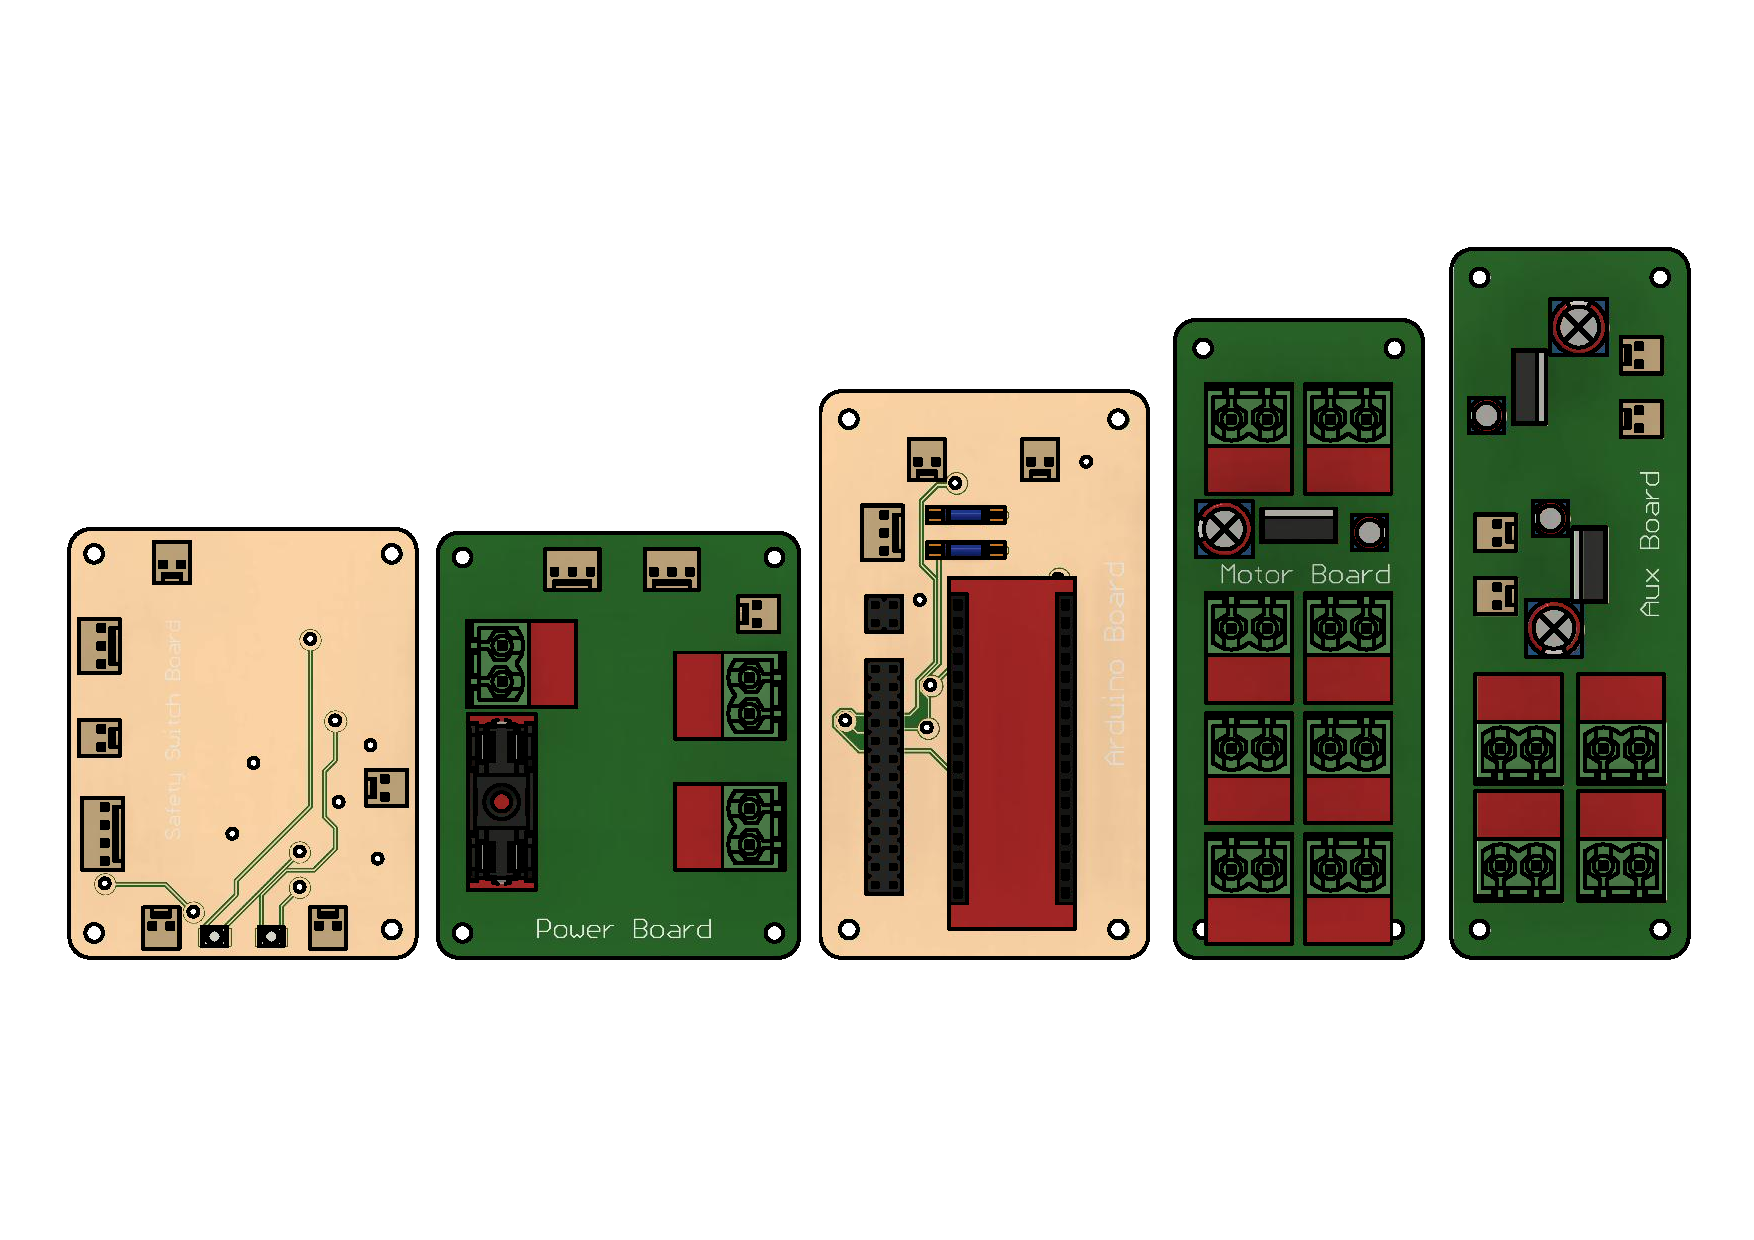
\includegraphics[width=1\textwidth]{Electronics/bulterpdb.pdf}
\caption{Top view of the boards in the PDB. From left to right: Safety Switch Board, Power Board, Arduino Board, Motor Board and Aux Board. The green areas are copper free areas and the red areas indicate connector clearance.}
\label{fig:butlerpdb}
\end{figure}

\subsubsection{Design}
The overall design to split the PDB into several boards has been chosen to simplify manufacturing and fault detection. This means that any issue is isolated to a single board and errors are more easily found. For complete specification of the boards see the manual. 

The Power Board is the main board that all power runs through. The power can be turned off with a main switch and the switching is done with MOSFETs\footnote{Metal–Oxide–Semiconductor Field-Effect Transistor}. The board has a fuse of 16 A installed to limit the maximum current. The Power Board has two power outputs controlled by the Safety Switch Board. The first output is the Motor output and it can supply a maximum of about 11 A. The second output is the auxiliary output and it can supply a maximum of about 10 A. 

The power is controlled from the Safety Switch Board. It controls the power to the outputs either from the main power switch or the safety switches. The board has four switches. The first switch is the main switch which controls the main power on or off. The second switch is a emergency switch which can disable the motors but having the control electronics enabled. The third switch is a magnetic switch that complements the emergency switch. A magnetic field need to be applied in the range of the magnetic switch to enable it. The fourth and last switch needs a "HIGH" digital signal in order to be enabled, this is controlled by the Arduino Board.
All switches are connected to an AND gate and needs to be "HIGH" for the Motor output to be enabled. In addition the Safety Switch Board as two LEDs, one green and one red, that indicate the status of the board. Green indicates that the board is on and all outputs are enabled and red indicates that at least one safety switch is not enabled so the motor output is disabled. Only one LED can be lit at the time.

The Motor Board is connected to the Power board and is basically an extension of the Power board. It has six outputs that use the battery voltage and two outputs that are regulated by a linear regulator at 12 V.

The Aux Board works by the same principle as the Motor board But is connected to the auxiliary output from the Power Board. It has four outputs that use the battery voltage and two 5 V and two 12 V linearly regulated outputs.

The Arduino board uses an Arduino Micro and communicates via I\textsuperscript{2}C bus connected to the Power Board were the voltage/current monitor is mounted. The Arduino Micro is programmed to monitor the voltage and current, this is to keep track of the voltage in order to determine when discharging of the battery should stop in order to protect the battery. The Arduino can then disable one of the safety switches which would disable the motors and the red LED will be lit. The Arduino board have been designed to be versatile with the pins from the Arduino Micro accessible for future functions.

\subsubsection{Future work}
The PDB have not been tested with the motors and the electronics, the only test that have been conducted is basic functionality. The PDB have not been wired on the Butler.

A battery have not been bought but the PDB was designed with the intention of using a LiFePO\textsubscript{4} battery from Biltema\footnote{\url{http://www.biltema.se/sv/}}. That battery have a voltage range of about 12.9 V to 14 V. If another battery with voltage below 12.9 V is going to be used, modifications need to be made to the PDB this is stated in the manual.

\subsection{System architecture - Ali Mokdad}
\begin{figure}[ht!]
\centering 
\includegraphics[width=1\textwidth]{Electronics/diagram.png}
\caption{Butler system architecture}
\label{fig:Butler system architecture}
\end{figure}

The system architecture of the Butler with the power requirements is shown in Figure~\ref{fig:Butler system architecture}. 
Table~\ref{table: The different motors for the Butler} lists brief explanation of each of the motors of the Butler.

\begin{table}[h!]
\centering
  \begin{tabular}{ | p{2cm}| p{9cm} |}
    \hline
    M1 arm  & Stepper motor for the first joint of the Butler arm   \\ \hline
    M2 arm  & Stepper motor for the second joint of the Butler arm   \\ \hline
    M3 arm  & Servo motor for rotating the hand. The feedback present in the diagram includes position, temperature, load, input voltage, etc.   \\ \hline
    M4 base & Dc motor with screw for moving all the arm up and down.\\ \hline
    M5 base & Stepper motor (same as M2 arm), for rotating the base of the Butler.\\
    \hline
  \end{tabular}
\caption{The different motors for the Butler}
\label{table: The different motors for the Butler}
\end{table}

\begin{table}[ht!]
\centering
  \begin{tabular}{ | p{2cm}| p{3cm} |}
    \hline
    M1 arm  & 14V, 0.4A    \\ \hline
    M2 arm  & 14V, 1.7A    \\ \hline
    M3 arm  & 12V, 2.2A    \\ \hline
    M4 base & 14V, 950 mA  \\ \hline
    M5 base & 14V, 1.7A    \\ \hline
    Cortex M4f & 5V        \\ \hline
    Jetson TX2 & 12 to 14V \\ \hline
  \end{tabular}
\caption{ Power requirements for the Butler}
\label{table: Power requirements for the Butler}
\end{table}

In the butler system: The PDB is responsible of providing power for the whole system. The Jetson TX2  is a full-featured development platform for visual computing, which constitutes the brain of the Butler; it communicates through a CAN bus with the Cortex M4f processor placed on a TM4C123G board which is an evaluation platform used for controlling the motors by sending the required PWM signals and serial communication (for the servo M3 hand) received from the Jetson TX2.
The LIDAR\cite{lidar} detection system which uses light from a laser to measure the distance to the object by illuminating that target with a pulsed laser light and send the data via USB communication to the Jetson TX2.
The Orbbec Astra Pro camera\cite{Camera} constitutes the eyes of the Butler, and the CHARLIE platform which is a different project platform will be used for this project. 
    \section{Mechanical Structure - Per Ekstr\"om}

One of the most fundamental parts of any robot is the mechanical structure, since the mechanical structure defines and limits the robot in what it can achieve physically. Below, the mechanical structure and the thought process behind it is described in great detail.

\subsection{Requirements}

Since the butler is supposed to compete at the RoboCup@HOME challenge\cite{robocup-rulebook}, the mechanical design will at the very least have to meet the requirements of that challenge. The relevant rules are:

\begin{itemize}
    \item The robot's internal hardware (electronics and wiring) must be covered up in an appealing way.
    \item Absolutely \textbf{no} duct tape on the outside!
    \item There may not be any loose cables hanging out of the robot.
    \item The robot may not have any sharp edges or other defects that could result in injury, human or otherwise.
    \item No constant annoying loud noises or blinding lights.
    \item The robot should not exceed the dimensions of a standard door (200cm x 70cm).
    \item There is no specific weight limit, but the robot should be lightweight enough for the participating team to be able to carry it off-stage in case of failure.
    \item The robot must have an emergency stop button and a speaker output plug.
\end{itemize}

% Describe the mechanical requirements for the competition here

\subsection{Previous work}

Previous year students have also attempted to build a butler, and the original plan was to build upon their work. However, the butler mechanical platform was inherited in such a state it could not be used to achieve the goals set for this project.

\subsubsection{Platform}

\begin{figure}[!ht]
    \centering
    \includegraphics[width=0.75\textwidth]{Mechanical_Structure/old-butler-platform.jpg}
    \caption{The platform the previous year students built.}
    \label{fig:old_butler_platform}
\end{figure}

The platform designed by previous year students was a low, sturdy and very bulky square base plate with four wheels, see figure \ref{fig:old_butler_platform}. The general design worked as advertised, but the platform is so heavy it cannot pass a bigger cable or threshold, and it also moves very slowly. The width also makes it difficult to pass through a regular door frame, though not impossible.

\subsubsection{Torso}

\begin{figure}[!ht]
    \centering
    \includegraphics[width=0.75\textwidth]{Mechanical_Structure/old-butler-arm-torso.jpg}
    \caption{The left image is the torso the previous year students built, while the right image is the 6 DOF arm.}
    \label{fig:old_butler_arm_torso}
\end{figure}

The torso on the old butler was very basic, but filled it's function remarkably well, see figure \ref{fig:old_butler_arm_torso}. It had one degree of freedom, up and down, but the lowest point is sitting quite a ways up, which meant that the butler could not reach and grasp things at the floor, at least not without a very long arm.

\subsubsection{Arm}

The arm on the old butler can be seen in figure \ref{fig:old_butler_arm_torso}. While the arm has six degrees of freedom and is built with a very sturdy frame, it was very bulky and would be difficult to encase within plastic, which is a requirement of the competition. It also failed the width requirement, since the arm made the robot have a total width of 80 cm even before a casing would have been added. This meant the robot would not be able to fit through a standard doorway.

Further complicating the issue, the robot arm was quite inaccurate as described in the report, and the weight was very heavy. It was also somewhat inaccurate, and the screws needed to be adjusted every fifth run or so. In conclusion, the arm would not make it into the competition in its current state.

\subsubsection{Gripper}

\begin{figure}[!ht]
    \centering
    \includegraphics[width=0.75\textwidth]{Mechanical_Structure/old-butler-gripper.jpg}
    \caption{The gripper the previous year students built.}
    \label{fig:old_butler_gripper}
\end{figure}

A gripper prototype has been developed by previous year students, see figure \ref{fig:old_butler_gripper}. Initially it was thought this gripper should merely be mounted to the old butler. After some further research it was concluded that the gripper is currently inadequate at gripping any type of round object, like a ball or cup of coffee, and is not suitable for the purposes of this project. It is a good proof of concept to show the gripping mechanisms and algorithms developed, but a new version must be developed.

\subsection{Design}

\begin{figure}[!ht]
    \centering
    \includegraphics[width=0.75\textwidth]{Mechanical_Structure/butler-overview.PNG}
    \caption{An overview of the finished butler design once mounted to the Husqvarna lawn mower. The actual work performed has been on the tower-like structure.}
    \label{fig:butler_overview}
\end{figure}

Given the requirements and considerations from above, two options presented themselves. One was to build upon the work of previous year students, and the other one was to start over. Given that a full redesign would have to be made at some point in time in either case to fulfil the goals of the competition, the decision was made to start over completely and take the hit this year rather than continuing to chase after an unrealistic goal. In this section, the design choices and general thinking of the final design will be presented. The final design can be found in figure \ref{fig:butler_overview}.

\subsubsection{Design goals}

The new butler has been designed with several key aspects in mind. It should be easy to modify, so that later year students can rework any part of the design, but also so that there is easy access to engines and other parts. It should also be lightweight, yet built to be durable and last a very long time.

The new butler frame has been designed to be able to carry a payload of at least 5 kg, but in practice the motors are the limiting factor here. The frame itself is designed to weigh no more than 20 kg and the robot platform has been tested to hold and operate for at least 24 kg. Since the empty platform itself weigh 7 kg, this means the robot should weigh no more than 30-35 kg in total.

The robot frame should also be designed for internal wiring from the get-go, since it is much easier to hide wires in a robot that was designed for it from the beginning.

And finally the butler should be designed for ease of manufacturing and use as much off-the-shelf parts as possible. This is mainly to save time, which is the most precious resource in this project, but also because off-the-shelf parts have already been tested for durability and safety requirements.

\subsubsection{Inspiration}

\begin{figure}[!ht]
    \centering
    \includegraphics[width=0.75\textwidth]{Mechanical_Structure/toyota-hsr.jpg}
    \caption{The Toyota HSR robot that was used as inspirational base for this robot.}
    \label{fig:toyota_hsr}
\end{figure}

The main inspiration for this robot has come from the Toyota HSR as shown in figure \ref{fig:toyota_hsr}. The HSR is the platform for the Domestic Standard Platform League in the competition. It has a single arm and is quite capable, though the new platform has a much more simple but robust arm. This is because we have no rotational joints, only hinge style joints, which makes it easier to fixate the arm and provides a much more robust operation.

Much of the inspiration also comes from industrial robotics and industry arms, but the decision was made to place as many motors as possible outside the arm in order to make it more lightweight, and control the second link through a driving belt from the base instead.

There were some preliminary research into HERB \cite{Srinivasa2009} for the gripper mechanics but due to time constraints, nothing ever came of it.

% Toyota robot
% HERB
% inMoov
% Pepper

\subsubsection{Platform}

At the base of the butler robot, there is a Husqvarna mobile autonomous lawnmower, with the top removed and replaced with a base plate made of transparent plastic. This allows for drilling holes and attaching mount points without having to worry about damaging or destroying the Husqvarna base.

The base in and of itself is very capable, and is tested to be able to carry loads of 25 kg. It is manoeuvred by two driving wheels operated with a differential drive, with two swivel caster wheels in the front for extra support.

\subsubsection{Torso}

\begin{figure}[!ht]
    \centering
    \includegraphics[width=0.75\textwidth]{Mechanical_Structure/turn_plate_mechanics.PNG}
    \caption{The mechanics design of the gear housing. The turnplate is on top of the axial bearing layer, with two engines driving the turn plate and ball screw respectively. The big gear im the middle drives the ball screw, the outer spur gear drives the turntable mechanism and the smaller gears are mounted to the engines and actually provide the motion required.}
    \label{fig:turn_plate_mechanics}
\end{figure}

The torso is built mostly from purchased parts, and have two degrees of freedom. At the bottom, there is a cylindrical gear box casing that house some gears which drives the turntable and ball screw, see figure \ref{fig:turn_plate_mechanics}. On top of that is a Lazy Susan style axial bearing layer\footnote{http://nomo2011.auderis.se/Default.asp?page=nyheter\_arkiv\_visa.asp\&wer=58} which produces nearly friction-free circular motion, and then the turn plate upon which everything else is mounted.

\begin{figure}[!ht]
    \centering
    \includegraphics[width=0.75\textwidth]{Mechanical_Structure/butler_arm_base_plate.PNG}
    \caption{The mechanics design of the arm base plate. The large motor in the back, m1, drives the first arm link and the outer part of the joint while the smaller motor m2 drives the inner part of the joint and, through a belt, also the second link movement.}
    \label{fig:arm_base_plate}
\end{figure}

In the middle of the turn plate, there is a ball screw that drives a plate up and down. This plate is where the arm is attached, see figure \ref{fig:arm_base_plate}. On the sides, four C-rails provide guidance and stability to the entire design, providing a smooth vertical motion that allows the arm to move up and down. Everything is tied together at the top with a plate that offers stability to the whole construction.

This design is very lightweight, yet still heavy enough to provide a sturdy and stable base of which to perform lifts from. It is also quite simple in it's design, which is great because simple is easy to understand and easy to expand and build.
    
% Rotating base plate
% C-rails
% Ball screw
% Gear housing in base

\subsubsection{Arm}

The arm can be divided into two sections - first and second link - and both are driven from the base plate in the middle of the elevator, according to figure \ref{fig:arm_mechanics}. It offers two degrees of freedom and is attached to the base plate by two ball bearing layers. Another set of ball bearing layers connect the first link to the second one, and both links are driven with gear belts from the base plate.

\begin{figure}[!ht]
    \centering
    \includegraphics[width=1.0 \textwidth]{Mechanical_Structure/butler_arm.PNG}
    \caption{The mechanical design of the arm. The image to the top left depicts how the arm base joint is put together, with the double axis mechanism, as well as the belt pulleys. The image to the top right shows the design of the second joint, which is controlled by the belt pulley. Finally the bottom image shows how the entire arm is assembled and put together. Not shown are the threaded rods that binds the arm together.}
    \label{fig:arm_mechanics}
\end{figure}

The two links are both held together by threaded rods, a design that also allows for adjusting any smaller imperfections that may arise. The second link is fastened by a cap, which makes sure the axis of the second link is centred. Similarly, the second link drive axis in the base may be adjusted if the need arises.

Both arm links are designed to be very lightweight, and use a lattice structure to achieve this work. This is also the reason the engines are placed outside the arms themselves, so they can be more lightweight.

% Three degrees of Freedom
% First and second degree from the same base
% Lightweight

\subsubsection{Gripper}

A decision was made to delay the gripper until the other parts were made. Unfortunately, this meant the gripper could not be designed, nor implemented in this project. Hopefully this can be sorted out in the future by others. The gripper should be able to rotate like a wrist, but only a basic design has been done during the project, and it has not been implemented.

\subsection{Implementation}

\begin{figure}[!ht]
    \centering
    \includegraphics[width=0.75\textwidth]{Mechanical_Structure/measurements.png}
    \caption{The final version for various relevant measurements for the butler robot. The travel distance is for the first axis of the first arm link.}
    \label{fig:final_version}
\end{figure}

\begin{figure}[!ht]
    \centering
    \includegraphics[width=0.75\textwidth]{Mechanical_Structure/final_result.jpg}
    \caption{The final version of the new butler torso and arm, with everything on it assembled.}
    \label{fig:mechanical_measurements}
\end{figure}

Building and implementing this construction with five degrees of freedom is not a small task. Due to the way it is constructed, extra care has to be taken on having precise measurements. In some parts, especially the turntable base part, there is very little room for error. Care has been taken in the design to allow for some adjustments of the imperfections that arise, but still provide a solid and rigid structure.

The work took a while to get started, but once the design part was over and done with and manufacturing and assembly started, things did move fairly quickly. The first focus was on getting the arm built, but it quickly became apparent that the arm base plate had to be manufactured and assembled first, and due to that limitation, the torso also had to be manufactured.

Going over the torso, it took several iterations to come up with the current design. It was decided early on to use C-rails for steering and a ball screw for moving the robot up and down, which give the robot a very rigid structure for the torso. 

Some parts of the design did not fall into place until later. In particular, gears had to be ordered and accounted for, as did placement of the engines. This lead to a few problems in fitting the gearing with what was already available.

Also, while implementing the design, the decision was made to break several complex parts into more easily manufactured pieces. This is something that should have been thought of from the start, but did not really effect the project as a whole.

As for materials, most of the parts are manufactured in milled aluminium or bent steel plates. A couple of parts are created by milled plastic, and the motor mounts were created in the 3D printer. However, a new iteration of the 3D printed parts must be created since their durability leaves a bit to be desired.

Unfortunately there were no time to implement the wrist joint, which is the biggest part left for future projects.

For the appropriate final measurements, see figure \ref{fig:mechanical_measurements}. As for the gear exchange ratios, these can be seen according to table \ref{table:gearing}.

\begin{table}[!ht]
    \centering
    \begin{tabular}{l l r r r}
        \multicolumn{1}{c}{\bfseries Joint} & \multicolumn{1}{c}{\bfseries Motor} & \multicolumn{1}{c}{\bfseries Driving} & \multicolumn{1}{c}{\bfseries Receiving} & \multicolumn{1}{c}{\bfseries Ratio} \\ %\hline
        First link belt & m1 & 30 & 30 & 1:1 \\
        Drive axis & m2 & 15 & 30 & 2:1 \\
        Drive axis belt & m2 & 19 & 19 & 1:1 \\
        Ball screw & m4 & 20 & 40 & 2:1 \\
        Turn plate & m5 & 20 & 80 & 4:1
    \end{tabular}
    \caption{The gearing exchanges for the various joints. Columns driving and receiving refers to the number of teeth on the driving gear vs the receiving gear.}
    \label{table:gearing}
\end{table}

% FEMA analysis
% Calculations
% Manufacturing process
% No third DOF

\subsection{Discussion}

\begin{figure}[!ht]
    \centering
    \includegraphics[width=1.0\textwidth]{Mechanical_Structure/new_joints.png}
    \caption{The implemented joints vs the new, improved and more easy to manufacture joints. The left side show the current joints and the right side show the improved joints. This change requires new link frames to be manufactured, however. At the top, the first link is shown and at the bottom is the second link.}
    \label{fig:new_joints}
\end{figure}

The biggest problem faced in the mechanics department was the lack of direction during the first five weeks of the project. Since the decision had not yet been set of whether or not a complete overhaul should be attempted, the mechanics department was stuck with a difficult decision to either work on what already existed, or start over from scratch, and this took a lot of time to evaluate.

The project started with the arm, something that, in hindsight, may not have been the best move. The arm frame was quickly built and manufactured, but in doing so, the project also locked itself in a certain solution which may not have been the best move. In particular, it was very hard to then come up with a satisfying solution to the arm base axis and moving the arm in a way that prevented it from slipping and gliding. This was eventually solved with glue. A better solution has now been designed as can be seen in figure \ref{fig:new_joints} but has yet to be manufactured and tested.

Apart from that, most of the things work just fine. The structure is rigid for the most part, which was one of the goals, but the middle joint on the arm is a bit loose. This issue can be solved by a slight redesign of the axis, but it has not been done due to time constraints.

One slight miss is that the gear controlling the ball screw axis is a bit wobbly, due to not having the proper axis dimensions (12mm instead of 10mm). This has been rectified by 3D-printing a part and adding more stop screws, but there is still a slight wobble.

The goal of being lightweight was one area where the project excelled. The entire butler frame, engines and all, weigh in at only 14.5 kg, and the stripped down base adds an additional 7.5 kg to that, bringing the total current weight to only about 22 kg - well below expectations. This is however without cabling, sensors and circuit boards mounted, so the total weight will be around 30 kg all in all.

One lesson learned is to start researching gears and other mechanical parts that you are going to buy first, and build your design from that. The workshop in Eskilstuna is powerful and can provide with a lot of help, but it cannot do everything.

Another thing that was noticed during the course of the project is that since the motor driving the second link is not attached to the arm, turning the first link will also turn the second link. This can however be corrected either in software or through a special drive mode in the electronics side.

Quite a few minor issues with the arm base platform and arm attachment remains. Had this project kept on for a couple more weeks, these issues would have undoubtedly been taken care of, but as it stands, it is not quite good enough. For the turntable base, everything works with the exception of the inner spur gear being slightly too high by a millimetre or two. This can be easily fixed by lowering the spur gear slightly, for instance by milling an indentation in the bottom plate. 

As for the rest of the issues, almost all of them have to do with the base plate not being large enough for the motors. A new version should be designed and manufactured, perhaps stacking the motors on top of each other.

On a final note, it is very important to double-check that the measurements of the data sheet are the same as the measurements in the real world. A couple of engine measurements were wrong here, but nothing a few extra holes and a little redesign could not fix.


% Everything works as intended
% A few parts needs adjustments
% Ball screw axis
% First link axis
% Second link axis cap
% Inaccurate data sheets

\subsection{Future work and conclusions}

Like any project, there will always be things to improve upon. Below is a list of the most prominent improvements, in no particular order. 

\begin{itemize}
    \item Cables must be drawn
    \item Circuit board mounts have yet to be designed
    \item Camera mount for the stereo camera has to be designed, but mounting holes exist
    \item Improve the middle joint of the arm
    \item Building a case for the entire construction frame
    \item A new gripper must be designed and manufactured
    \item The arm base plate should be redesigned from the ground up, placing the motors in a better fashion
    \item Drive belts must be tightened up somehow
    \item The frames for the first and second link in the arm should be remade with the new design for the joints
\end{itemize}

Hopefully these improvements will be able to get done by others in the future. In conclusion, there are a lot of improvements to be made, but the mechanical platform also holds a lot of promise for the future.


% \newpage

%Suggestions for subsections - don't forget to include calculations that has been made.

%\subsection{Introduction/Background}
%\subsection{Requirements}
%\subsection{Overview}
%\subsection{Design}
%Motivate design - reference inspirations
%\subsection{Implementation}
%\subsection{Conclusions/future work/discussion}

    
\section{Electronics - Ali Mokdad}
The electronics department constitutes a link between programming and mechanical structure, by establishing the movement of the mechanical parts of the Butler with respect to the code. This section declares the electronic components used in the Butler project including the motors, motor controllers and development boards.

\subsection{Motors and gearboxes - Ali Mokdad}  \label{MotorsNGearboxes}


\subsubsection{Requirements}
The actuators of the Butler have been chosen with respect to mechanical calculations based on the weight of the Butler arm to choose the correct motors according to two main parameters: Torque and speed. The calculations have been divided in two parts: The first part is concerning the different parts of the arm of the Butler, and the second part is concerning the base of the Butler. 

\begin{enumerate}
\item \textbf{Calculations for the arm:}\\
The arm of the Butler is connected to the base from the shoulder part, where a metal plate holding the motors M1 and M2 constitutes the link between the arm and the base of the Butler.
The arm of the Butler consists of three parts: A shoulder joint rotated by M1 arm, an elbow joint rotated by M2 arm and a wrist rotated by M3 arm. Note that M2 arm is located next to M1 arm in order to make the arm lighter. Figure~\ref{fig:Arm structure of the Butler}  represents the weight distribution considered for the arm:

\begin{figure}[h!]
\centering
\captionsetup{justification=centering}
\includegraphics[width=1\textwidth]{Electronics/arm.jpg}
\caption{Arm structure of the Butler where M2 arm is located next to M1 arm in order to make the arm lighter}
\label{fig:Arm structure of the Butler}
\end{figure}


The maximum mass of the whole arm  is:

\begin{equation} \label{eq:m_total}
\begin{split}
M_{total} & = m1 + m2 + m3\\
& = 0.5 + 0.3 + 1\\
& = 1.8 Kg\\
\end{split}
\end{equation}

In order to calculate the torque needed for each motor, the centre of mass of the parts needed to be lifted by each of the motors needs to be calculated, by taking the position of each motor as the origin (when X=0).
The Centre of mass is calculated by the following equation:

\begin{equation} \label{eq: X_cm}
\begin{split}
X_{cm} & = \frac{m_1*X_1 + m_2*X_2 + m_3*X_3}{m_1 + m_2 + m_3} \\ 
\end{split}
\end{equation}
Where X1, X2 and X3 are the distances from the motor position (origin) to the centre of gravity of each part of the arm.\\

\begin{itemize}

\item \textbf{For M1 arm}: 
\begin{equation} \label{eq: X_Cm1}
\begin{split}
X_{Cm1} & = \frac{(0.15*0.5) + (0.4*0.3) + (0.6*1)}{0.5 + 0.3 +1} \\
& = 0.44
\end{split}
\end{equation}


 
The torque needed from M1 arm is:
\begin{equation} \label{eq: T_M1}
\begin{split}
T_{NeededM1} & = X_{Cm1} *  M_{total} * gravity\\
& = 0.44 * 1.8 * 9.82\\
& = 7.8 Nm\\
\end{split}
\end{equation}

\item \textbf{For M2 arm:} \\
The center of mass needed for M2 arm is:
\begin{equation} \label{eq: X_Cm2}
\begin{split}
X_{Cm2} & = \frac{(0.4*0.3) + (0.2*1) }{0.3 + 1}  \\
& = 0.246
\end{split}
\end{equation}

The torque needed from M2 arm is:
\begin{equation} \label{eq: T_M2}
\begin{split}
T_{NeededM2} & = X_{Cm2}*  M_{afterElbow} * gravity\\
& = 0.246 * (0.3+1) * 9.82\\
& = 3.13 Nm\\
\end{split}
\end{equation}

\item \textbf{For M3 arm:} \\
The center of mass needed for M3 arm is:
\begin{equation} \label{eq: X_Cm3}
\begin{split}
X_{Cm3} & = \frac{(0.1*1)}{1} \\
&= 0.1
\end{split}
\end{equation}

The torque needed from M3 arm is:
\begin{equation} \label{eq: T_M3}
\begin{split}
T_{NeededM3} & = X_{Cm3} *  M_{afterWrist} * gravity\\
& = 0.1 * 1 * 9.82\\
& = 0.982 Nm\\
\end{split}
\end{equation}

\end{itemize}

\item \textbf{Calculations for the base}:\\
The base of the butler consists of two motors: M4 base and M5 base. The motor M4 base is responsible of moving the whole arm of the butler up and down, by rotating a screw attached to a spindle, enabling the arm to move over the axis which is in this case the spindle. The motor M5 base is responsible of making the base of the butler rotate, resulting in a change of the direction.\\

\textbf{For M4 base:}
The selection of the motor M4 base has been fully referred to mechanical requirements based on two major factors: the force produced by the weight of the arm over the motor, and the lead of the spindle attached to a screw. According to calculations made in the mechanics section, the major requirement of the motor M4 base is the speed. The needed speed is 50 Rpm as a minimum with a torque of 0.2 Nm to 0.3 Nm as maximum.
\\

\textbf{For M5 base}
The motor M5 base requires low torque and low speed, in order to rotate the base of the Butler.

\end{enumerate}
In order to make the Butler as efficient as possible, the followings assumptions have been made:
\begin{itemize}
    \item The motors M1 arm, M2 arm, M5 base should be stepper motors since high precision and high torque is required respectively in rotating the whole arm, rotating the elbow joint and rotating the base of the Butler.
    \item The motor M3 arm should be a servo motor, since servos provide extreme precision (but lower torque than stepper motors).
    \item The motor M4 base should be a DC motor since high speed is needed, to be able to rotate the screw fast enough to reach the requirement of 50 RPM as speed of the motor.
\end{itemize}





%%%%%%%%%%%%%%%%%%%%%%%%%%%%%%%%%%%%%%%%%%%%%%%%%%%%%%%%%%%%%%%%%%%%%%%%%%%%%%%%%%%%%%%%%%%%%

\subsubsection{Motors and gearboxes selection}
In order to achieve the motor requirements, the following motors and gear boxes have been chosen:
\\
\begin{enumerate}
    \item \textbf{M1 arm: Rotating the the whole arm of the Butler:}\\\\
    \textbf{Motor:}
    \begin{itemize}
        \item Name: planetary gear unipolar stepper motor\cite{m1}.
        \item Nominal voltage: 9.6 V.
        \item Current: 0.4 A.
        \item Nominal torque: 0.086 Nm.\\
    \end{itemize}
    
    \textbf{Gearbox:}
    \begin{itemize}
        \item Gearbox type: Planetary.
        \item Reduction ratio: 104:1.
        \item Backlash at no-load: less than 1.5 degrees.\\
    \end{itemize}
    
    \textbf{Motor with gearbox:}
    \begin{itemize}
        \item Name: planetary gear unipolar stepper motor.
        \item Weight: 740 g.
        \item Price: 440.46 SEK.
        \item Part number: RB-Dyd-02.
        \item Supplier: Robotshop.
     \end{itemize}
    In order to know if the motor M1 arm combined with the gearbox will be able to carry the weight of the arm, the maximum output torque needs to be calculated. 
    From the specifications above of the motor M1 arm, the maximum output torque is:\\
    \begin{equation} \label{eq: T_M1arm}
    \begin{split}
    T_{M1arm} & = T_{Motor} * R_{max}\\
    & =  0.086 * 104\\
    & = 8.944 Nm\\
    \end{split}
    \end{equation}
    Where T\textsubscript{M1arm} is the maximum output torque of the motor M1 arm, T\textsubscript{Motor} is the nominal torque of the motor without the gearbox, and R\textsubscript{max} the reduction ratio from the gearbox.
    
    In addition, a mechanical gear attached to the motor could modify the final values. The mechanical gear having a reduction ratio of 1:1 for this motor remains the same as the following calculations show:
    \begin{equation} \label{eq: T_M1Final}
    \begin{split}
    T_{M1Final} & = T_{M1arm} * R_{mechanical}\\
    & =  8.944 * 1\\
    & = 8.944 Nm\\
    \end{split}
    \end{equation}
    
    Where T\textsubscript{M1Final} is the final output torque after mechanical gearing, T\textsubscript{M1arm} is the output torque of M1 arm, and R\textsubscript{mechanical} is the reduction ratio of the mechanical gear.
    
    The above combination shows that the output torque of M1 arm (8.944 Nm) exceeds the required torque (7.8 Nm), making the motor chosen sufficient for rotating the arm of the Butler.\\
   
%%%%%%%%%%%%%%%%%%%%%%%%%%%%%%%%%%%%%%%%%%%%%%%%%%%%%%%%%%%%%%%%%%%%%%%%%%%%%%%%%%%%%%%%%%%%%%%%%%%%%%%%%%
    \item \textbf {M2 arm: Rotating the the elbow of the Butler:}\\
    \textbf{Motor:}
    \begin{itemize}
        \item Name: NEMA-17 bipolar stepper motor\cite{M2andM5}.
        \item Nominal voltage: 12 V.
        \item Current: 1.7 A.
        \item Nominal torque: 0.047 Nm\\
       
    \end{itemize}
    
    \textbf{Gearbox:}
    \begin{itemize}
        \item Gearbox type: Planetary.
        \item Reduction ratio: 99.5:1.
        \item Backlash error: 1.5 degrees.\\
    \end{itemize}
    
     \textbf{Motor with gearbox:}
    \begin{itemize}
        \item Name: NEMA-17 bipolar stepper motor with planetary gearbox.
        \item Weight: 564 g.
        \item Price: 801.60 SEK.
        \item Part number: RB-Phi-267.
        \item Supplier: Robotshop.
    \end{itemize}
    
     From the specifications above of the motor M2 arm, the maximum output torque is:\\
    \begin{equation} \label{eq: T_M2arm}
    \begin{split}
    T_{M2arm} & = T_{Motor} * R_{max}\\
    & =  0.047 * 100\\
    & = 4.7 Nm\\
    \end{split}
    \end{equation}
    
    A mechanical gear having a reduction ratio of 2:1 attached to M2 arm modifies the output torque value, as shown below:
    
    \begin{equation} \label{eq: T_M2Final}
    \begin{split}
    T_{M2Final} & = T_{M2arm} * R_{mechanical}\\
    & = 4.7 * 2\\
    & = 9.4 Nm\\
    \end{split}
    \end{equation}
    
    Since the final output torque of M2 arm (9.4 Nm) is higher than the required torque (3.13 Nm), the motor is assumed to be sufficient for rotating the elbow of the Butler.\\
    
%%%%%%%%%%%%%%%%%%%%%%%%%%%%%%%%%%%%%%%%%%%%%%%%%%%%%%%%%%%%%%%%%%%%%%%%%%%%%%%%%%%%%%%%%%%%%%%%%%%%%%%    
    \item \textbf {M3 arm: Rotating the wrist of Butler:}\\\\
   \textbf{Motor:}
    \begin{itemize}
        \item Name: AX18-a dynamixel servo motor\cite{servo}.
        \item Operating voltage: 9 to 12 V.
        \item Current: 2.2 A.
        \item Nominal torque:0.007 Nm.\\
    \end{itemize}
    
    \textbf{Gearbox:}
    \begin{itemize}
        \item Gear built in with the motor.
        \item Gear ratio: 254:1.\\
    \end{itemize}
    
    \textbf{Motor with gearbox:}
    \begin{itemize}
        \item Name: AX18-a dynamixel servo motor.
        \item Weight: 54.5 g.
        \item Price: 792.42 SEK.
        \item Part number:RB-Rbs-101
        \item Supplier: Robotshop. 
    \end{itemize}
    
    According to the specifications above of the motor M3 arm, the maximum output torque is:\\
    \begin{equation} \label{eq: T_M3arm }
    \begin{split}
    T_{M3arm} & = T_{Motor} * R_{max}\\
    & =  0.007 * 254\\
    & = 1.77 Nm\\
    \end{split}
    \end{equation}
    The output torque of M3 arm (1.77 Nm) is higher than the required torque (0.982 Nm), which means that the motor chosen is sufficient. This motor is not attached to a mechanical gear so the output remains the same.\\
    
    
%%%%%%%%%%%%%%%%%%%%%%%%%%%%%%%%%%%%%%%%%%%%%%%%%%%%%%%%%%%%%%%%%%%%%%%%%%%%%%%%%%%%%%%%%%%%%%%%%%%%%%%


    \item \begin{itemize}
        \item  \textbf {M4 base: Rotating a screw attached to a spindle to move all the arm of the Butler:}\\\\
   \textbf{Motor:}
    \begin{itemize}
        \item Name:  Lynxmotion brushed DC gear motor\cite{M4}.
        \item Nominal voltage: 12 V.
        \item Current: 250 mA.
        \item Nominal torque: 0.034 Nm.\\
    \end{itemize}
    
    \textbf{Gearbox:}
    \begin{itemize}
        \item Gear Ratio: 5.2:1.\\
    \end{itemize}
    
    \textbf{Motor with gearbox:}
    \begin{itemize}
        \item Name: Lynxmotion brushed DC gear motor.
        \item Weight: 533 g.
        \item Price: 714.04 SEK.
        \item Part number: RB-Wtc-02.
        \item Supplier: Robotshop.\\
    \end{itemize}
    
    The specifications above result in the following maximum output torque:
    \begin{equation} \label{eq: T_M4base}
    \begin{split}
    T_{M4base} & = T_{Motor} * R_{max}\\
    & =  0.034 * 5.2\\
    & = 0.1768 Nm\\
    \end{split}
    \end{equation}
    
    The output torque obtained (0.1768) compared to the required torque (0.2 to 0.3 Nm) is not enough; But the use of a mechanical gear having a reduction ratio of 50:12 made the values approved, the motor M4 base attached to the mechanical gear resulted in an output torque of:
    \begin{equation} \label{eq: T_M4Final}
    \begin{split} 
    T_{M4Final} & = T_{M4base} * R_{mechanical}\\
    & =  0.1768 * 4.166\\
    & = 0.73 Nm\\
    \end{split}
    \end{equation}
    
    
    The output speed of the motor M4 base is:
    
    \begin{equation} \label{eq: Speed_M4base}
    \begin{split}
    Speed_{M4base} & = speed_{Motor} / R_{max}\\
    & =  2496 / 5.2\\
    & = 480 Rpm\\
    \end{split}
    \end{equation}
    
    The output speed of the motor attached to the mechanical gear is:
    
    \begin{equation} \label{eq: Speed_M4Final}
    \begin{split} 
    Speed_{M4Final} & = Speed_{M4base} / R_{mechanical}\\
    & =  480 / 4.166\\
    & = 115.21 Nm\\
    \end{split}
    \end{equation}
    
    The final output speed obtained (115.21 Rpm) exceeds the demanded speed (50 Rpm), making the motor M4 base chosen approved.\\
    
    \item \textbf{Encoder: Hall effect encoder YC2010}\\
    In order to detect the position and the speed of the motor M4 base, an encoder is required. A \textbf{hall effect encoder YC2010} attached to the motor M4 base gives feedback about the motor position by detecting a change in voltage by magnetic deflection of electrons. The encoder consists of a 2 channel output A and B that are 90 electrical degrees out of phase, which enables direction sensing. The YC2010 encoder consists of the following wires:
    \begin{itemize}
        \item \textbf{Red wire:} Powering up the motor (+).
        \item \textbf{Black wire:} Powering up the motor (-).
        \item \textbf{Green wire:} Hall sensor GND.
        \item \textbf{Blue wire:} Hall sensor VCC.
        \item \textbf{Yellow wire:} Hall sensor channel A Vout.
        \item \textbf{White wire:} Hall sensor channel B Vout.\\
    \end{itemize}
   
    
    \end{itemize}
    
%%%%%%%%%%%%%%%%%%%%%%%%%%%%%%%%%%%%%%%%%%%%%%%%%%%%%%%%%%%%%%%%%%%%%%%%%%%%%%%%%%%%%%%%%%%%%%%%%%%%%%%   
    \item \textbf {M5 base: Rotating the base of the Butler:}\\\\
     \textbf{Motor:}
    \begin{itemize}
        \item Name: NEMA-17 bipolar stepper motor with planetary gearbox\cite{M2andM5}.
        \item Nominal voltage: 12 V.
        \item Current: 1.7 A.
        \item Nominal torque: 0.047 Nm.\\
    \end{itemize}
    
    \textbf{Gearbox:}
    \begin{itemize}
        \item Gearbox type: Planetary.
        \item Reduction ratio: 99.5:1.
        \item Backlash error: 1.5 degrees.\\
    \end{itemize}
    
    \textbf{Motor with gearbox:}
    \begin{itemize}
        \item Name: NEMA-17 bipolar stepper motor with planetary gearbox.
        \item Weight: 564 g.
        \item Price: 801.60 SEK.
        \item Part number: RB-Phi-267.
        \item Supplier: Robotshop.\\
    \end{itemize}
    
    This motor has been chosen after considering that the weight of the Butler will not be held by this motor, in fact the weight will be held by the base platform (i will reference this). 
    This motor has been chosen because of the lack of time, which made choosing an already available motor a must, since the shipping needs time. This motor has the following output torque:
    
    \begin{equation} \label{eq: T_M5base}
    \begin{split}
    T_{M5base} & = T_{Motor} * R_{max}\\
    & =  0.047 * 100\\
    & = 4.7 Nm\\
    \end{split}
    \end{equation}
    
    A mechanical gear having a reduction ratio of 80:20 attached to M5 base modifies the output torque value, as shown below:
    
    \begin{equation} \label{eq: T_M5Final}
    \begin{split}
    T_{M5Final} & = T_{M5base} * R_{mechanical}\\
    & = 4.7 * 4\\
    & = 18.8 Nm\\
    \end{split}
    \end{equation}
\end{enumerate}


%%%%%%%%%%%%%%%%%%%%%%%%%%%%%%%%%%%%%%%%%%%%%%%%%%%%%%%%%%%%%%%%%%%%%%%%%%%%%%%%%%%%%%%%%%%%%

\subsubsection{Price and weight}
The sum of the price and weight for all the motors with the gearboxes are listed below:\\\\
\textbf{Price:} 3550.12 SEK.\\\\
\textbf{Weight:} 2455.5 grams. 

\subsubsection{Conclusion}
The motors chosen for the Butler showed good performance. However, their performance did not reach the expectations desired, where data-sheet values were not fully reached like the torque and speed for example, due to their low cost.
As future work, the motors would be replaced by Maxon Motors, in case of high budget availability, where detailed selection of motor with compatible gearbox and encoder is available with fully explained data-sheets.
%%%%%%%%%%%%%%%%%%%%%%%%%%%%%%%%%%%%%%%%%%%%%%%%%%%%%%%%%%%%%%%%%%%%%%%%%%%%%%%%%%%%%%%%%%%%%%%%%%%%%%%%%%%%%%%%%%%%%%%%%%%%%%%%%%%%%%%%%%%%%%%%%%%%%%%%%%%%%%%%%%%%%%%%%%%%%%%%%%%%%%%%%%%%%%%%%%%%%%%%%%%%%%%%%%%%%%%%%%%%%%%%%%%%%%%%%%%%%%%%%%%%%%%%%%%%%%%%%%%%%%%%%%%%%%%%%%%%%%%

\subsection{Motor controllers - Ali Mokdad}
\label{MotorController}%Do not remove please.
% \subsubsection{Introduction}
In order to control the motors, a motor controller needs to be used. A motor controller enables modifying the speed and the direction of rotation of the motor. Basically, every motor needs a controller to be able to control its performance as desired by the user.

%%%%%%%%%%%%%%%%%%%%%%%%%%%%%%%%%%%%%%%%%%%%%%%%%%%%%%%%%%%%%%%%%%%%%%%%%%%%%%%%%%%%%%%%%%%%%

\subsubsection{Requirements}
The motor controllers for the Butler were chosen with respect to the motor selection process. There are two major types of motor controllers: Stepper motor controller and DC motor controller. For the Butler, since the chosen motors are three stepper motors and one DC motor, then there should be three stepper motor controllers (for the motors M1 arm, M2 arm and M5 base) and one DC motor controller (for the motor M4 base).\\
In addition, the motor controllers should be able to handle the current needed by each motor. For the Butler, two \textbf{stepper} motor controllers should handle 1.7 Amps, and one last stepper motor controller should handle 0.9 Amps. The \textbf{DC} motor controller should handle 0.25 Amps.
%%%%%%%%%%%%%%%%%%%%%%%%%%%%%%%%%%%%%%%%%%%%%%%%%%%%%%%%%%%%%%%%%%%%%%%%%%%%%%%%%%%%%%%%%%%%%
\subsubsection{Motor controllers selection}

In order to fulfill the requirements, the selected motor controllers are: a TB6600\cite{Gpu2017} stepper motor driver and an MD30C\cite{ppp} DC motor driver. Three of the TB6600 stepper motor driver have been used for controlling the three stepper motors M1 arm, M2 arm and M5 base, and one MD30C DC motor driver for controlling the DC motor M4 base.\\
The TB6600 stepper motor driver replaced a Cytron SD02C\cite{123} stepper motor driver tested in the early stages of the project since this SD02C driver resulted in bad performance proving that it is not suitable for driving the selected motors. The conclusion section below states further explanation about the reason why the SD02C stepper motor driver has been replaced by the TB6600 stepper motor drive.

%%%%%%%%%%%%%%%%%%%%%%%%%%%%%%%%%%%%%%%%%%%%%%%%%%%%%%%%%%%%%%%%%%%%%%%%%%%%%%%%%%%%%%%%%%%%%

\subsubsection{Testing motor controllers}
For testing the motor controllers, the following connections needs to be established as shown in figure~\ref{Motor controller connection for testing}.
\begin{itemize}
    \item Connection for powering up the motor controller.
    \item Connection to the motor.
    \item Connection for a PWM signal.
    \item Connection for the direction of rotation.
\end{itemize}

\begin{figure}[h!]
\centering
\includegraphics[width=0.8\textwidth]{Electronics/controller.png}
\caption{Motor controller connection for testing}
\label{Motor controller connection for testing}
\end{figure}%% ALI CHECK CHAT



%%%%%%%%%%%%%%%%%%%%%%%%%%%%%%%%%%%%%%%%%%%%%%%%%%%%%%%%%%%%%%%%%%%%%%%%%%%%%%%%%%%%%%%%%%%%%

\subsubsection{Results and conclusions}
As a result of testing, the SD02C stepper motor driver did not reach the expected results during driving the motor. A strange sound was produced when using it for driving the motors which made the motor run in very low speed. The problem stated in the current that the SD02C stepper motor driver was able to handle, which is 1 A of continuous run; where the current needed by two of the stepper motors was 1.7 A.\\
For that reason, the SD02C stepper motor driver has been replaced by the TB6600 stepper motor driver, where the current needed can be controlled for enabling motors needing high current to be driven by this motor driver.
%%%%%%%%%%%%%%%%%%%%%%%%%%%%%%%%%%%%%%%%%%%%%%%%%%%%%%%%%%%%%%%%%%%%%%%%%%%%%%%%%%%%%%%%%%%%%%%%%%%%%%%%%%%%%%%%%%%%%%%%%%%%%%%%%%%%%%%%%%%%%%%%%%%%%%%%%%%%%%%%%%%%%%%%%%%%%%%%%%%%%%%%%%%%%%%%%%%%%%%%%%%%%%%%%%%%%%%%%%%%%%%%%%%%%%%%%%%%%%%%%%%%%%%%%%%%%%%%%%%%%%%%%%%%%%%%%%%%%%%

\subsection{Cortex-M4f - Ali Mokdad}
\label{CortexM4}
% \subsubsection{Introduction/Background}
The Cortex-M4f is a processor developed to address digital signal control markets that demand an efficient and easy to use combination of control and signal processing capabilities. The combination of high-efficiency signal processing functionality with the low-power, low cost and ease-of-use benefits of the Cortex-M family of processors is designed to satisfy solutions specifically targeting the motor control, automotive, power management, embedded audio and industrial automation markets.

\subsubsection{Requirements}
For the Butler project, communication between the different parts of the robot is a must. A development board capable of controlling the motors of the butler is needed. The Butler project is intended to have high efficiency where CAN communication is a requirement.

\subsubsection{Cortex-M4f development board TM4C123G}
In order to fulfil the conditions, a development board having CAN communication is demanded. The Cortex-M4f development board TM4C123G\cite{cor} has been chosen for controlling the motors by sending the specific PWM signal to the motor drivers. This development board features a 32-bit CORTEX M4F microcontroller and has the following specifications:
\begin{itemize}
    \item A clock speed of 80 MHZ which is enough for this project.
    \item 16 PWM outputs with 16-bit counter, which is enough for all the system.
    \item 2 CAN with bit rate up to 1 Mbit/s.
    \item In the CAN controller 11-bit identifier (standard) or a 29-bit identifier (extended) are supported.
    \item 8 UART peripherals.
    \item Real-time JTAG debugger.
    \item Uses C programmimg language.
\end{itemize}

\subsubsection{Conclusion}
The Cortex-M4f development board TM4C123G has been able to control the motors without showing any malfunction. As a result of that, the development board proved to be very efficient for the Butler project.
%%%%%%%%%%%%%%%%%%%%%%%%%%%%%%%%%%%%%%%%%%%%%%%%%%%%%%%%%%%%%%%%%%%%%%%%%%%%%%%%%%%%%%%%%%%%%%%%%%%%%%%%%%%%%%%%%%%%%%%%%%%%%%%%%%%%%%%%%%%%%%%%%%%%%%%%%%%%%%%%%%%%%%%%%%%%%%%%%%%%%%%%%%%%%%%%%%%%%%%%%%%%%%%%%%%%%%%%%%%%%%%%%%%%%%%%%%%%%%%%%%%%%%%%%%%%%%%%%%%%%%%%%%%%%%%%%%%%%%%

\subsection{Nvidia Jetson TX2 - Ali Mokdad}
% \subsubsection{Introduction/Background}
The NVIDIA Jetson TX2\cite{Board} Developer Kit is a full-featured development platform for visual computing. It is ideal for applications requiring high computational performance in a low power envelope. The Jetson TX2 Developer Kit comes pre-flashed with a Linux environment, includes support for many common APIs, and is supported by NVIDIA’s complete development tool chain. The board exposes many standard hardware interfaces, enabling a highly flexible and extensible platform.

\subsubsection{Requirements}
A developer kit with high computational performance was required to provide a "Brain" for the Butler which would be responsible of sending commands to the CORTEX M4f processor, and handle inputs from the LIDAR and the Orbbec Astra Pro camera. In addition, UART communication with the CHARLIE platform (which constitutes the base) is needed.
In order to achieve the demanded requirements, two developer kits were compared to choose the one more suitable for the Butler project and these developer kits are: The NIVIDIA Jetson TX2, and the NUC5i7RYH which uses an Intel i5 processor. Where the NIVIDIA Jetson TX2 has been chosen having more hardware interfaces than the NUC5i7RYH.

\subsubsection{Specifications}
The carrier Board of the Jetson TX2 has the following feature list:

\begin{itemize}
    \item Storage: Full Size SD Card Slot, SATA Connector (Power and TX/RX). 
    \item USB: USB 2.0 and USB 3.0 Type A.
    \item Display Expansion Header:
        \begin{enumerate}
            \item DSI (2x4 lanes).
            \item eDP/DP/HDMI.
            \item Backlight: PWM/Control.
            \item Touch: SPI/I2C.
        \end{enumerate}
    \item HDMI Type A. 
    \item Camera Expansion Header:
        \begin{enumerate}
            \item CSI: 6, x2 – 3, x4.
            \item Camera CLK, I2C and Control. 
            \item I2S, UART, SPI, Digital Mic.
        \end{enumerate}
    \item Expansion Header: I2C, SPI, UART, I2S, Audio Clock/Control, D-MIC.
    \item GPIO Expansion Header: I2S, GPIOs, Digital Speaker.
    \item Debug/Serial:
        \begin{enumerate}
            \item  JTAG Connector.
            \item  Debug Connector.
            \item  JTAG, UART, I2C, Power, Reset and Recovery.
            \item Serial Port Signals.
        \end{enumerate}
    \item Fan Connector: 5V, PWM and Tach.
    \item Power:
    \begin{enumerate}
            \item DC Jack: 5.5V-19.6V.
            \item Main 3.3V/5V Buck Supplies.
            \item Main 1.8V Buck Supply.
            \item USB VBUS Load Switches.
            \item  12V Boost (PCIe and SATA).
            \item Load Switches/LDOs (SD/HDMI/Display/Camera).
            \item Charge Control Header.
        \end{enumerate}
\end{itemize}

\subsubsection{Conclusion}
The NIVIDIA Jetson TX2 developer kit has proved itself having the required qualities to control the Butler project, which has been verified in the AI group testing only, since the project hasn't reach its final results to be tested as a full project.
%%%%%%%%%%%%%%%%%%%%%%%%%%%%%%%%%%%%%%%%%%%%%%%%%%%%%%%%%%%%%%%%%%%%%%%%%%%%%%%%%%%%%%%%%%%%%%%%%%%%%%%%%%%%%%%%%%%%%%%%%%%%%%%%%%%%%%%%%%%%%%%%%%%%%%%%%%%%%%%%%%%%%%%%%%%%%%%%%%%%%%%%%%%%%%%%%%%%%%%%%%%%%%%%%%%%%%%%%%%%%%%%%%%%%%%%%%%%%%%%%%%%%%%%%%%%%%%%%%%%%%%%%%%%%%%%%%%%%%%

% \section{Sensors - Billy Lindgren(move?)}
\subsection{Camera - Billy Lindgren}

\medskip

\noindent

For the robot to be able to avoid obstacles that are not detected by the LIDAR, a camera was mounted to the front of the robot. To be able to calculate a correct distance to the found hindrance some form of a stereo camera was needed to be used, either an active stereo camera or a passive one. The cameras that were under investigation were the ZED stereo camera from Stereolabs \cite{ZEDcamera} and Astra Pro from ORBBEC \cite{AstraPro}.

\subsubsection{Performance and Limitations of the ZED, a passive stereo camera}
\noindent
The ZED requires a USB 3.0 port and sends data at targeted device and has a frame rate at 100 fps with the quality 640x480 of the images. The data speed sets a limitation on the usage of the USB bus and it is preferred that the ZED is the only device on a USB port and not use a USB-hub to obtain more port.

A limitation is that the ZED draws power from the USB port that limits the usage of the Jetson and is limiting the use of USB-hubs significantly, thus only USB-hubs that have an external power source should be used to limit the power consumption from the Jetson. However, a USB-hub us not recommended at all, due to the amount of data the ZED provides through the bus. Since the ZED is a passive stereo camera it performs poorly in dark environments, due to the fact a ZED consists of 2 monocular cameras light is needed to get a clear picture.

\subsubsection{Performance and Limitations of Astra PRO, an active stereo camera}
\noindent
The data transfer speed of the Astra pro is 27Mb/s and it provides 30 fps with the quality 640x480. The quality can be set higher, but the frame rate will drop equally as much. i.e. if the quality is increased to 1280x720 the frame rate will be lowered to 10 fps. The difference is linear if the quality is 3 times higher the frame rate will be divided by 3.
 
Astra pro contains an IR-sensor and a monocular RGB camera. Since it uses an IR-sensor it performs poorly in sunlight due to noise that occurs when the sensor picks up the IR-beams the sun emits.
 
\subsubsection{Point Cloud Differences}
 
There is some differences between the point clouds from the cameras. The Astra Pro's point cloud is a more accurate point cloud and less sensitive due to the utilization of the IR-sensor to measure the depth in the image, while the RGB camera is used for gathering data of how the environment looks like. These sensor data are then fused into an accurate point cloud. The ZED point cloud
is in that manner more sensitive due to the fact that the ZED is 2 RGB cameras, whose images are overlapping to create a 3D image, by calculating the depth instead of measuring it. This makes the ZED more computational heavy due to more calculations than the Astra Pro and creates a less accurate point cloud.


\subsubsection{Discussion}
One can argue that one camera is the better than the other, but it depends on the environment the camera is going to operate in. Since the camera will operate in an ordinary indoor environment, the performance and requirements of the Astra Pro make it more preferable than the ZED. The ZED outperforms the Astra Pro though, in terms of video quality and frame rate and thanks to the high frame rate of the ZED, fast moving objects can be easier detected.

 
\subsubsection{Conclusion} 
It was concluded that the Astra Pro is more suited than the ZED for the Butler project due to the more sensitive and accurate point cloud that can be utilised for grabbing a cup in the sense of knowing how far away the cup is.  
 



% \subsection{Lidar}
% Why Lidar?
% About the SICK Lidar
% \subsubsection{Advantages}
% \subsubsection{Disadvantages}
% \subsection{Stereo Camera}
% Why Stereo Camera?
% About ZED
% \subsubsection{Advantages}
% \subsubsection{Disadvantages}
% \subsection{Ultrasonic Rangefinders}
% Why Ultrasonic Rangefinders?
% Ultrasonic Sensor System
% \subsubsection{Advantages}
% \subsubsection{Disadvantages}


%%%%%%%%%%%%%%%%%%%%%%%%%%%%%%%%%%%%%%%%%%%%%%%%%%%%%%%%%%%%%%%%%%%%%%%%%%%%%%%%%%%%%%%%%%%%%%%%%%%%%%

\subsection{CAN transceiver - Ali Mokdad} \label{CANtransceiver}

% \subsubsection{Introduction}
A CAN transceiver is a device that serves as the interface between a CAN protocol controller and the physical bus. A CAN transceiver always has two bus pins: one for the CAN high line (CANH) and one for the CAN low line (CANL). Each electronic component that needs to send or receive from the CAN bus needs to have a CAN transceiver. In this project, a high-speed CAN transceiver is used: The MCP2551 \cite{Types2010}. The MCP2551 provides differential transmit and receive capability for the CAN protocol controller and it will operate at speeds of up to 1 Mb/s. A board is designed for each of the components that need to send and receive from the CAN bus (The Jetson TX2 \cite{Board} and the cortex M4f \cite{She2013}), to fit on these two components.
For high-speed CAN communication, both ends of the pair of signal wires (CAN-H and CAN-L) must be terminated, to achive that, a resistor 120 ohm needs to be added on the board between CAN-H and CAN-L.



\subsubsection{MCP2551 layout}
The MCP2551 CAN transceiver is an IC component that consists of 8 pins as shown in figure~\ref{fig: MCP2551 CAN transceiver}. Table ~\ref{table: MCP2551 PINOUT} explains the pins of the CAN transceiver.
\begin{figure}[h!]
\centering
\includegraphics[width=0.3\textwidth]{Electronics/can.png}
\caption{MCP2551 CAN transceiver}
\label{fig: MCP2551 CAN transceiver}
\end{figure}

\begin{table}[h!]
\centering
  \begin{tabular}{ | p{2cm}| p{2cm} | p{5cm}|} 
    \hline
    1  & TXD  & Transmit Data Input \\ \hline
    2  & VSS  & Ground \\ \hline
    3  & VDD  & Supply Voltage\\ \hline
    4  & RXD  & Receive Data Output\\ \hline
    5  & Vref & Reference Output Voltage\\\hline
    6  & CANL & CAN Low-Level Voltage I/O\\\hline
    7  & CANH & CAN High-Level Voltage I/O\\\hline
    8  & Rs   & Slope-Control Input\\
    \hline
  \end{tabular}
\caption{MCP2551 PINOUT}
\label{table: MCP2551 PINOUT}
\end{table}

\subsubsection{Specifications}
\begin{itemize} 
    \item Supports 1 Mb/s operation.
    \item Implements ISO-11898 standard physical layer requirements.
    \item Suitable for 12V and 24V systems.
    \item Externally-controlled slope for reduced RFI emissions.
    \item Detection of ground fault (permanent Dominant) on TXD input.
    \item Power-on Reset and voltage brown-out protection.
    \item An unpowered node or brown-out event will not disturb the CAN bus.
    \item Low current standby operation.
    \item Protection against damage due to short-circuit conditions (positive or negative battery voltage)
    \item Protection against high-voltage transients.
    \item Automatic thermal shutdown protection.
    \item High-noise immunity due to differential bus implementation.\\
\end{itemize}

\subsubsection{Conclusion}
The CAN transceiver card achieved the expected outcome which consisted of enabling the CORTEX M4F and the NIVIDIA Jetson TX2 to send and receive data from the CAN bus. The transceiver card worked successfully for the CORTEX M4f  but not for the Jetson TX2. Since a pin has been connected wrong during the milling process (the error has been spotted in a late stage of the project), which resulted in disabling the communication for the Jetson TX2. Which proves that the transceiver card design worked (since it worked for the CORTEX M4f), and the error has been just in the milling process.

\subsection{Power Distribution Board - Alexander Falk}
The redesign of the Butler demanded new electronics and motors. This meant that a new Power Distribution Board (PDB) was needed. The PDB is one of the fundamental parts of the Butler since it supplies power to all the electronics and motors in order for the Butler to operate. See the manual on Teams for the comprehensive view of the components and layout\footnote{Butler PDB - butler\_pdb.pdf on Microsoft Teams}.
\subsubsection{Requirements}
The main requirements involve the correct voltage levels and current ratings. From the specifications, see table \ref{table: Power requirements for the Butler}, the voltage levels that is required are 5 V, 12 V and maximum 14 V. The motors together would require about 7 A. The Cortex M4f has an USB connector for the power and that is rated for a maximum of 500 mA at 5 V. The Jetson TX2 power adapter is rated 90 W and at 12 V equals 7.5 A.

Then there was requirements regarding safety. The Butler should be able to be stopped in case of an error. It was desired to have minimum of an emergency switch for the arm and a magnetic switch for the motors that drive the Butler forward.

The last requirement involve the ability to measure the voltage and current in order to see the utilisation and evaluate the performance.
\subsubsection{Overview}
The PDB for the Butler Project is designed to supply power to the motors and additional electronics. The PDB is divided in five separate boards (see figure \ref{fig:butlerpdb}): Power Board, Safety Switch Board, Motor Board, Aux (Auxiliary) Board and Arduino Board. The PDB have safety functions which enables the control electronics to be powered but having the motors disabled. The Power Board also has the ability to measure the voltage and current with a voltage/current monitor. The voltage/current Monitor communicates via I\textsuperscript{2}C bus connected to the Arduino Board. The Arduino Board is designed to have a Arduino Micro mounted and have all outputs available to facilitate different communication needs. All digital signals of the boards operate at 5 V logic levels.

\begin{figure}[ht!]
\centering 
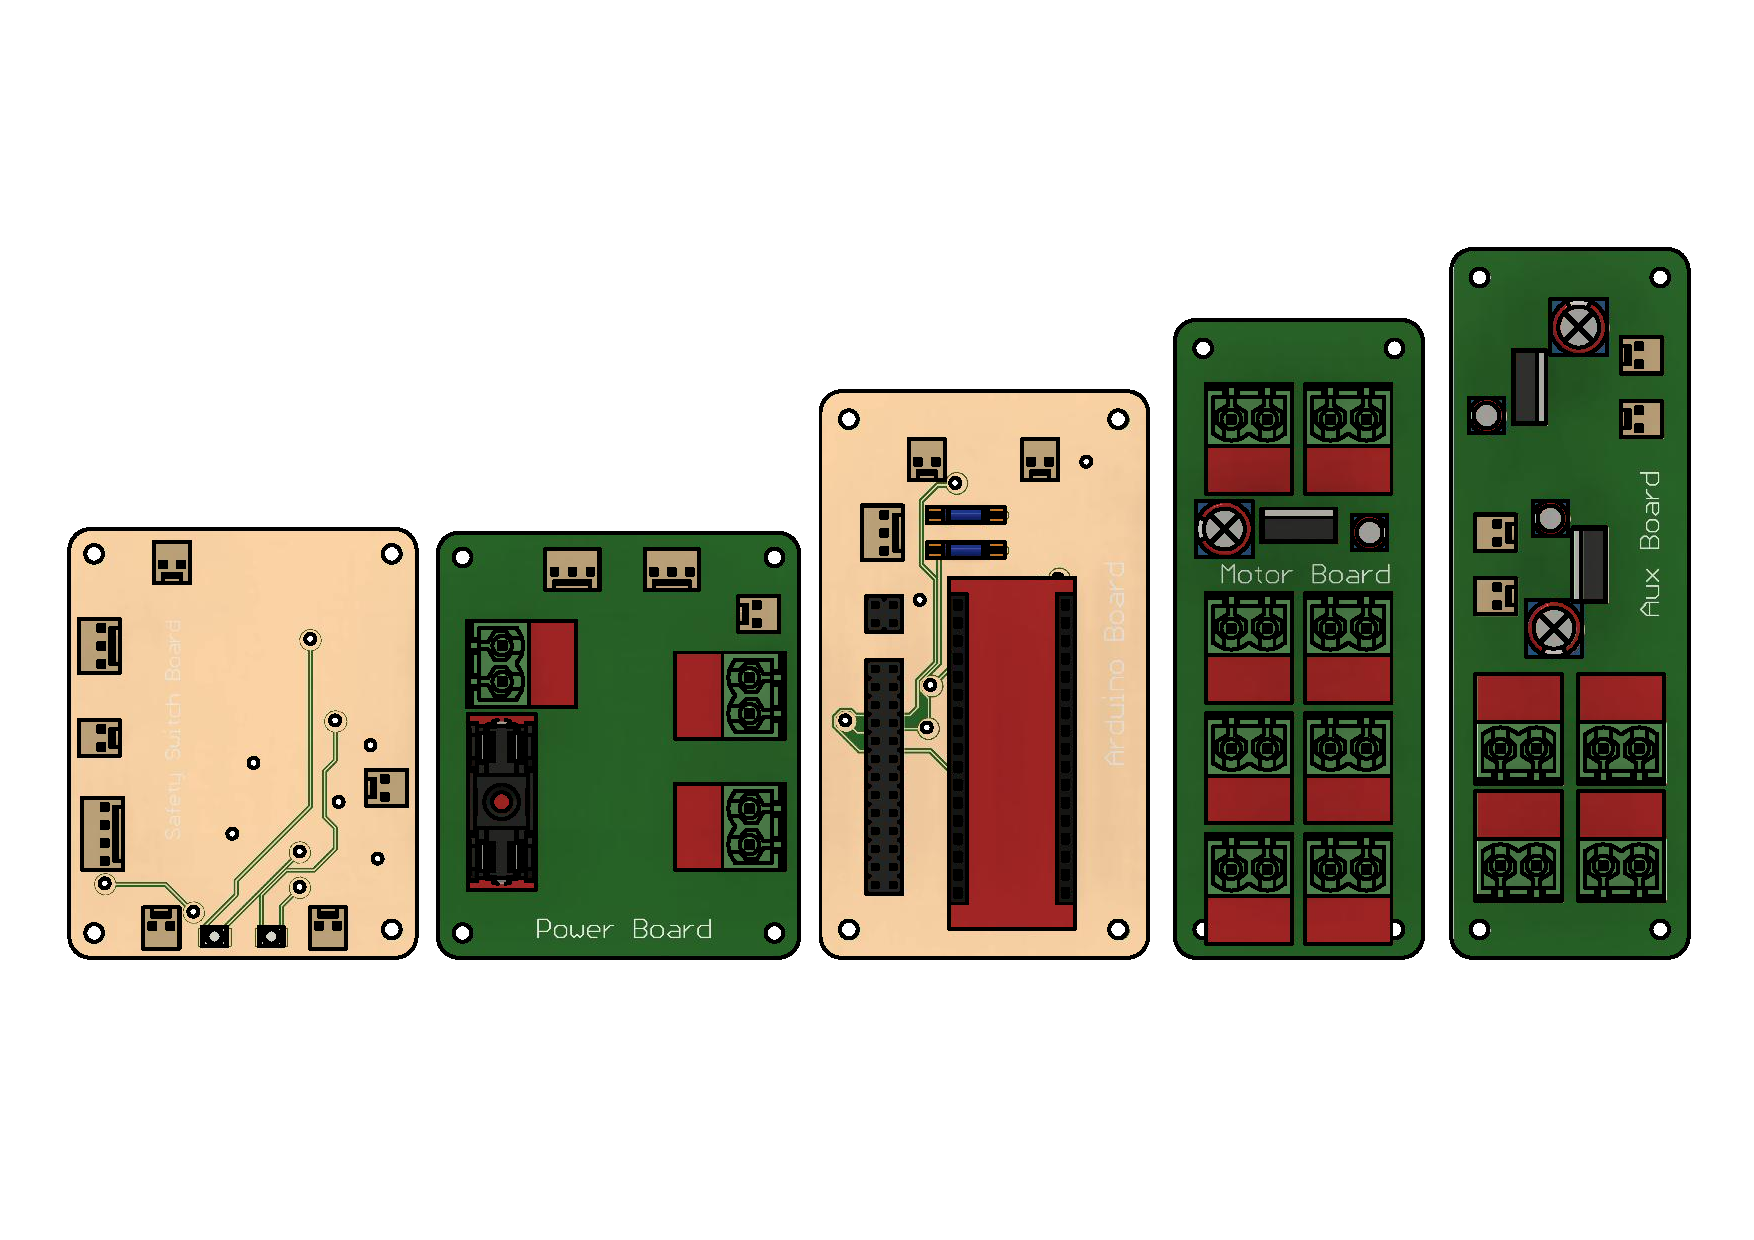
\includegraphics[width=1\textwidth]{Electronics/bulterpdb.pdf}
\caption{Top view of the boards in the PDB. From left to right: Safety Switch Board, Power Board, Arduino Board, Motor Board and Aux Board. The green areas are copper free areas and the red areas indicate connector clearance.}
\label{fig:butlerpdb}
\end{figure}

\subsubsection{Design}
The overall design to split the PDB into several boards has been chosen to simplify manufacturing and fault detection. This means that any issue is isolated to a single board and errors are more easily found. For complete specification of the boards see the manual. 

The Power Board is the main board that all power runs through. The power can be turned off with a main switch and the switching is done with MOSFETs\footnote{Metal–Oxide–Semiconductor Field-Effect Transistor}. The board has a fuse of 16 A installed to limit the maximum current. The Power Board has two power outputs controlled by the Safety Switch Board. The first output is the Motor output and it can supply a maximum of about 11 A. The second output is the auxiliary output and it can supply a maximum of about 10 A. 

The power is controlled from the Safety Switch Board. It controls the power to the outputs either from the main power switch or the safety switches. The board has four switches. The first switch is the main switch which controls the main power on or off. The second switch is a emergency switch which can disable the motors but having the control electronics enabled. The third switch is a magnetic switch that complements the emergency switch. A magnetic field need to be applied in the range of the magnetic switch to enable it. The fourth and last switch needs a "HIGH" digital signal in order to be enabled, this is controlled by the Arduino Board.
All switches are connected to an AND gate and needs to be "HIGH" for the Motor output to be enabled. In addition the Safety Switch Board as two LEDs, one green and one red, that indicate the status of the board. Green indicates that the board is on and all outputs are enabled and red indicates that at least one safety switch is not enabled so the motor output is disabled. Only one LED can be lit at the time.

The Motor Board is connected to the Power board and is basically an extension of the Power board. It has six outputs that use the battery voltage and two outputs that are regulated by a linear regulator at 12 V.

The Aux Board works by the same principle as the Motor board But is connected to the auxiliary output from the Power Board. It has four outputs that use the battery voltage and two 5 V and two 12 V linearly regulated outputs.

The Arduino board uses an Arduino Micro and communicates via I\textsuperscript{2}C bus connected to the Power Board were the voltage/current monitor is mounted. The Arduino Micro is programmed to monitor the voltage and current, this is to keep track of the voltage in order to determine when discharging of the battery should stop in order to protect the battery. The Arduino can then disable one of the safety switches which would disable the motors and the red LED will be lit. The Arduino board have been designed to be versatile with the pins from the Arduino Micro accessible for future functions.

\subsubsection{Future work}
The PDB have not been tested with the motors and the electronics, the only test that have been conducted is basic functionality. The PDB have not been wired on the Butler.

A battery have not been bought but the PDB was designed with the intention of using a LiFePO\textsubscript{4} battery from Biltema\footnote{\url{http://www.biltema.se/sv/}}. That battery have a voltage range of about 12.9 V to 14 V. If another battery with voltage below 12.9 V is going to be used, modifications need to be made to the PDB this is stated in the manual.

\subsection{System architecture - Ali Mokdad}
\begin{figure}[ht!]
\centering 
\includegraphics[width=1\textwidth]{Electronics/diagram.png}
\caption{Butler system architecture}
\label{fig:Butler system architecture}
\end{figure}

The system architecture of the Butler with the power requirements is shown in Figure~\ref{fig:Butler system architecture}. 
Table~\ref{table: The different motors for the Butler} lists brief explanation of each of the motors of the Butler.

\begin{table}[h!]
\centering
  \begin{tabular}{ | p{2cm}| p{9cm} |}
    \hline
    M1 arm  & Stepper motor for the first joint of the Butler arm   \\ \hline
    M2 arm  & Stepper motor for the second joint of the Butler arm   \\ \hline
    M3 arm  & Servo motor for rotating the hand. The feedback present in the diagram includes position, temperature, load, input voltage, etc.   \\ \hline
    M4 base & Dc motor with screw for moving all the arm up and down.\\ \hline
    M5 base & Stepper motor (same as M2 arm), for rotating the base of the Butler.\\
    \hline
  \end{tabular}
\caption{The different motors for the Butler}
\label{table: The different motors for the Butler}
\end{table}

\begin{table}[ht!]
\centering
  \begin{tabular}{ | p{2cm}| p{3cm} |}
    \hline
    M1 arm  & 14V, 0.4A    \\ \hline
    M2 arm  & 14V, 1.7A    \\ \hline
    M3 arm  & 12V, 2.2A    \\ \hline
    M4 base & 14V, 950 mA  \\ \hline
    M5 base & 14V, 1.7A    \\ \hline
    Cortex M4f & 5V        \\ \hline
    Jetson TX2 & 12 to 14V \\ \hline
  \end{tabular}
\caption{ Power requirements for the Butler}
\label{table: Power requirements for the Butler}
\end{table}

In the butler system: The PDB is responsible of providing power for the whole system. The Jetson TX2  is a full-featured development platform for visual computing, which constitutes the brain of the Butler; it communicates through a CAN bus with the Cortex M4f processor placed on a TM4C123G board which is an evaluation platform used for controlling the motors by sending the required PWM signals and serial communication (for the servo M3 hand) received from the Jetson TX2.
The LIDAR\cite{lidar} detection system which uses light from a laser to measure the distance to the object by illuminating that target with a pulsed laser light and send the data via USB communication to the Jetson TX2.
The Orbbec Astra Pro camera\cite{Camera} constitutes the eyes of the Butler, and the CHARLIE platform which is a different project platform will be used for this project. 
    \section{CAN communication - Giancarlo Kuosmanen}
Controller Area Network (CAN) is a serial communication protocol. The CAN protocol supports real-time controls with a high level of security. Some of the main areas of application that CAN extends to are high-speed networks to low cost multiplex wiring. It simplifies electrical wiring systems and reduces faults greatly, as demonstrated by the author Robert Bosch\cite{bosch}. CAN high-speed reaches speeds of up to 1 Mbit/s, while low speed goes from 125kbit/s which is the downside of low-speed, but the upside is that it contains a fault-tolerant system. It is fault-tolerant in the sense that, if the signal gets cut in one wire or shorted to ground, it can still continue to process messages\cite{Kvaser}.
CAN is defined by the ISO standard (11898), mentioned in e.g Bosch\cite{bosch}. Already mentioned protocols are high-speed CAN (11898-2) and low-speed CAN (11898-3). CAN follows the Open System Interconnect (OSI)\footnote{\url{http://www.axiomatic.com/whatiscan.pdf}} model of computer communication architecture that is subdivided into different layers:

\begin{itemize}
    \item Transfer layer and object layer handles all the functionality of the data link layer. Finding which message is going to be transmitted, received messages and message prioritisation. It also provides the interface on the message structure.
    \item Physical layer is the actual transfer between different CAN nodes connected to NUC (bare bone PC) or PC and embedded systems, varies depending on the system and CAN transceivers are a part of the physical layer, detailed in the CAN transceiver section, i.e \ref{CANtransceiver}.
\end{itemize}

The card that was used in this project is Texas Instruments TM4C123GXL, with its specifications mentioned in section  \ref{CortexM4}, paired up with the Texas Instruments TM4C123GH6PM \cite{TexasInstruments} controller. It conforms to CAN protocol versions 2.0A and 2.0B. Version 2.0A has a 11 bit-identifier (Standard CAN) and 2.0B has a 29 bit-identifier (Extended CAN) headers and Transfer rates up to 1 MBit/s \cite{TexasInstruments}. The header gives the possibility to transmit messages with different identifiers, this way its easier to control, and enables the ability to prioritise the messages.\newline  With a high bandwidth and low message count in addition to low number of nodes connected to the system. Protocol 2.0A will do with its 11 bit-identifier. The TM4C123GH6PM controller has a CAN protocol controller that uses message objects. The message object holds the current information, status and data of the transferred message. It has a set of 32 memory blocks for both transmitting and receiving messages. It further provides the ability to send with 32 different ID's.\newline
\indent In this project, the high-speed CAN was selected due to the ability of for sending messages in short amounts of time. The 2.0A header was selected due to few nodes connected to the CAN bus also, the utilisation of the 11-bit identifier is plenty sufficient for the intended task. CAN and its features with message identifiers make the system more versatile in a way that if the system needs to be expanded, by adding another MCU (Micro Controller Unit), no radical change has to be made, though the receiving end must be adjusted to fit the new id admission.
%%%%%%%%%%%%%%%%%%%%%%%%%%%%%%%%%%%%%%%%%%%%%%%%%%%%%%%%%

\subsection{Test Scenarios} 
The testing phase was divided into three parts. \newline
\begin{itemize}
    \item First part: Shows how the circuitry was made and which components are needed for a successful CAN communication.
    \item Second part: Kvaser Leaf Light HS cable\footnote{\url{https://www.kvaser.com/product/kvaser-leaf-light-hs/}} substitutes a TM4C123GXL card for sniffing purposes and sending specific CAN messages.
    \item Concluding phase: Replaces the PC to Jetson and is connected to a MCU.
\end{itemize}
\subsubsection{Scenario 1}

The goal was to enable the CAN communication between the two cards. A simple transmitting and receiving program was implemented. For it to work completely, two CAN transceivers were needed, paired up with two \(120\Omega\) resistors, as depicted in figure~\ref{fig:CANcom}. Transceivers are needed for the physical layer if it is to work. The MCUs have on-board CAN controllers. The CAN bus operates with a TTL (Transistor-Transistor Logic), 5 volt as high and 0 volt as low. This logic does not generate the needed differential signal(CAN-High and CAN-Low) for the CAN bus. Therefore, transceivers are included. The two resistors placed at the end of the bus are tasked with removing signal reflection and ensure that the bus gets the correct voltage levels. With this setup, the communication worked as intended. By using a terminal program, the UART from the card could print out its values and progress on the command window which Hercules\footnote{Terminal program specifically for hardware} engendered, shown in figure~\ref{fig:Hercules}.
\begin{figure}[!ht]
\centering
\includegraphics[width=0.75\textwidth]{Communication/CANoverlay.png}
\caption{Electrical circuit for the CAN communication between two TM4C123GXL cards.}
\label{fig:CANcom}
\end{figure}
%%%%%%%%%%%%%%%%%%%%
\begin{figure}[!ht]
\centering
\includegraphics[scale=0.35]{Communication/Hercules.png}
\caption{Hercules software.}
\label{fig:Hercules}
\end{figure}
%%%%%%%%%%%%%%%%%%%%%%%%%%%%%%%%
\subsubsection{Scenario 2}

In this scenario a TM4C123GXL card was replaced with a Kvaser Leaf Light HS cable shown in figure \ref{fig:KvaserToMCU}, paired up with the software CANKing\footnote{\url{https://www.kvaser.com/canking/}}. The Kvaser Leaf Light HS cable uses a standard 9-pin D-Sub Connector (RS-232) shown in figure \ref{fig:KvaserLeafPinHead}. CANKing makes it possible to send specific data in each message. It controls the interface of the CAN and gives an overview with the output window. The output window shows received and transceived messages. It also shows what kind of data they contain. CANKing is the pseudo replacement for Jetson. If this system works as intended then it should work with Jetson.\newline
\indent During the development and testing of this period of time a successful system was produced. The controller for the motors worked and so did the CAN communication.
\begin{figure}[!ht]
\centering
\includegraphics[width=0.5\textwidth, keepaspectratio]{Communication/KvaserToMCU.png}
\caption{Replaced one TM4C123GXL card for Kvaser Leaf Light HS cable. Remove one transceiver (MCP2551) and couple the Kvaser CANH and CANL to the pins onto the MCP2551 CANH and CANL. Kvaser pinout shown in figure~\ref{fig:KvaserLeafPinHead}}
\label{fig:KvaserToMCU}
\end{figure}
%%%%%%%%%%%%%%%%%%%%%%%%%
\begin{figure}[!ht]
\centering
\includegraphics[width=0.25\textwidth]{Communication/KvaserLeafPinHead.png}
\caption{Shows the pinouts for the Kvaser RS-232. The most important pins are CANH and CANL. Picture available at: \url{http://www.kvaser.com/software/7330130980146/V1_2_189/kvaser_leaf_light_v2_usersguide.pdf}.}
\label{fig:KvaserLeafPinHead}
\end{figure}
%%%%%%%%%%%%%%%%%%%%%%%%
\subsubsection{Scenario 3} 
The PC was replaced by a Jetson, shown in figure \ref{fig:FinalStage}. \newline 
When sniffing (debugging) with the Kvaser cable and CANKing, messages were being transmitted and received. Instead of correct CAN messages, the receiver received Error Frames. Error frames indicate that the communication is operating but with corrupt messages. This may occur when the system does not have the correct speed at both ends. Adjusting the speed of the messages in Jetson was an intricate task.  \newline
\begin{figure}[!ht]
\centering
\includegraphics[width=0.25\textwidth]{Communication/FinalStage.png}
\caption{Communication between Jetson TX2 and TM4C123GXL}
\label{fig:FinalStage}
\end{figure}
% \newpage
%%%%%%%%%%%%%%%%%%%%%%%%%
\subsection{Motor control - Alexander Karlsson \& Giancarlo Kuosmanen}
\label{motorcancontrol}
\begin{figure}[!ht]
\centering
\includegraphics[width=0.65\textwidth]{Communication/Motor_Control.png}
\caption{Motor control flowchart.}
\label{fig:Motor_Control}
\end{figure}
Three stepper motors are controlled by a single interrupt (triggered by a timer). The position of stepper motors are known from the amount of pulses generated and the position of DC motor is computed using an encoder. Tasks are created with FreeRTOS\footnote{\url{https://www.freertos.org/}} for the receiver, transceiver, stepper control, and dc control (PID). The transceiver task is called when motors are done generating the pulses requested by the Jetson and then suspends itself (by looking at the number of messages in the transceivers' message queue). The message queue is used in the stepper control task to handle one command at a time (also waits for the transceiver task to complete).
\newline
\indent Stepper motors are controlled by the bytes\footnote{One byte represents 255 in decimal form} in the CAN message, two dedicated bytes for each motor, can be seen in figure \ref{fig:CANKingMessage}. DC motor only needs one byte. First byte is for pulses, 1.8 degree steps, also controls the direction of the motor. The  second byte is for micro-stepping, in increments of 1.8/16 degrees and 1.8/32. %Inserting CANKing picture here soon!
A value of 100 stops the motor, below 100 makes the motor rotate CCW (Counter clock wise) and values over 100 makes the motor rotate CW(Clock-wise). Utilising 100 as the indicator of controlling the direction. \newline \indent Each stepper motor has its micro-stepping driver, mentioned in Section \ref{MotorController}, which restricts the use of the motor. Generation of PWM (Pulse Width Modulation) signals from MCU had its limitations with the drivers.\newline \indent The two smaller (M2 and M5) stepper motors in Section \ref{MotorsNGearboxes} had their drivers set on 16 micro-steps and a PWM which has a frequency of 20kHZ . The larger (M1, mentioned in Section \ref{MotorsNGearboxes}) stepper motor had its driver set on 32 micro-steps and a PWM of 20kHZ. Frequencies above 20kHZ made the motor to stop functioning properly. For the smaller ones, a PWM above 30kHZ caused problems and the motor could not rotate. \newline 
\indent Boundaries found were from examining and testing each stepper motor. The reason for these limitations remains unclear. The DC motor(M4) has its own driver which demands a 20kHZ PWM signal, no problems were encountered with the DC driver nor with the motor.  
\begin{figure}[!ht]
\centering
\includegraphics[width=0.65\textwidth]{Communication/CANKingMessage.png}
\caption{CANKing message structure. How the bytes are divided among the motors. Data byte field enables the byte field.}
\label{fig:CANKingMessage}
\end{figure}
\subsection{CAN and ROS communication - Albin B}
%abn1213\\
Communication between ROS and the motors was done using CAN. Several packages were used to do this, the main one being ros\_control which handles when and what to communicate to the motors. The second package is called ros\_canopen which handles transferring messages to the motors using the CAN bus. The message structure for each message consists of 8 bytes of data and a message ID. The message ID is currently irrelevant since there is only one type of message that can be sent. The 8 data bytes are divided into 4 different parts, one for each motor and each part contains values for ticks and micro ticks which is how many degrees we want the motor to move.

Ticks range from 0-200 and each tick is 360/200=1,8 degrees where 100 is zero degrees and anything below 100 is negative degrees. So if we send 99 ticks we want the motor to move -1,8 degrees and 101 is +1,8 degrees. So the maximum range of movement that the CAN message can communicate to the motors is -180 to 180 degrees. Micro ticks are for finer adjustments, one micro tick is tick(1,8)/32=0.05625 degrees. The values for micro ticks in the CAN message ranges from 0-32. Micro ticks are always added to degrees meaning micro ticks can't be negative. So if ticks are 98=-1,8*2=-3,6 and micro ticks are 16 0.05625*16=1,8/2=0,9 then we are telling the motor to move negative 3,6 degrees and then add the micro ticks onto that so the final result would be -2,7 degrees. For positive ticks it would be 102=1,8*2=3,6 and then you add the 16 micro ticks 3,6+0.05625*16=4,5 degrees.

The ros\_control package has sparse documentation but the ros\_control\_boilerplate package helped greatly for implementation and our code for CAN communication was added to this package. There is currently only an implementation for writing to the CAN bus and no implementation for reading from the CAN bus which would have to be done if the motors are to give feedback to the ros\_control package. See the documentation for more details on how the code works.

\begin{table}[!ht]
\centering
\caption{CAN message data structure}
\label{my-label}
\begin{tabular}{|c|c|c|c|c|c|c|c|}
\hline
\multicolumn{2}{|c|}{Motor 1} & \multicolumn{2}{c|}{Motor 2} & \multicolumn{2}{c|}{Motor 3} & \multicolumn{2}{c|}{Motor 4} \\ \hline
Ticks       & Micro ticks      & Ticks      & Micro ticks      & Ticks      & Micro ticks      & Ticks      & Micro ticks      \\ \hline
\end{tabular}
\end{table}



\subsection{Future Work} 
The PID-controller for the DC motor works as intended but recently discovered that if there is a burst of messages, the PID controller gets unstable. It works when the messages come within $~$0.2 sec gaps. It has something to do with the calculation not having enough time to finish before the next message arrives so an if-statement can secure the issue.\newline After the motors have finished its task, the MCU sends back a statement to the Jetson containing the current position of the stepper motors but not for the DC motor. Including the DC motor into the message interface could be necessary but since the ROS controller in the Jetson does not take the DC into consideration, it provides pulses which is not optimal. The DC motor wants longer distances to move otherwise the PI-controller will create unnecessary overshoots at times, this part could be developed further. To recap it short and concise.
\begin{itemize}
  \item Include the DC motor into the CAN message on the transceiving end of the TM4C123GXL card.
  \item Improve the collaboration between Jetson and the MCU. Avoid sending pulses and micro-pulses to the DC engine due to the PI-controller and its overshoot problems. Rather give it a smaller distance for it to move. 
  \item Optional - Bit-shifting could be a better solution instead of using whole bytes, makes the system more versatile. Enables more options and properties, control the speed, pulses, acceleration and direction. At the moment the system only manages to control direction and pulses.
  \item The CAN data field has 8 bytes in total, only 7 bytes are being utilised. 1 byte remains and can be used for any given motor. 
\end{itemize}

%%%%%%%%%%%%%%%%%%%%%%%%%%%%%%%%%%%%%%
%\subsection{Requirement}   %Requirements is included in the design of the circuit as well as the testing part.
%\subsection{Overview}      %A brief overview will be given when explanations of the scenarios are given.
%\subsection{Design}        %Will include pictures on the circuitry - Could also show the ultiboard design for the break out card?
%\subsection{Implementation}%Implementation will be given in the motor controller. 


    \section{Development and Simulation Tools}
\subsection{ROS - Alexander Karlsson, Niclas Holmqvist}
The Robot Operating System\footnote{\url{http://www.ros.org/}} (ROS) is an open-source (BSD) collection of libraries and tools for developing robotic systems \cite{quigley2009ros}, where the main idea is to be able to reuse code for different purposes and contribute new innovations to the community. The core functionality is built around a peer-to-peer network of processes called "nodes" that communicates with each other by sending messages with the help of a master, which provides services such as name registration and lookup-tables in the network. These messages may be advertised as a topic or a service who shares some similarities but are very different. In both cases the name of the topic/service is used to identify its contents on the network but they are based on different semantics, where the topics are built around publishing and subscribing. A topic may be compared to a bus where anyone connected to it is able to access the messages and multiple nodes may subscribe to the same topic at one time. In comparison a service is based around requesting and replying where the request may be comprised of a different message type than the reply. The connection between nodes is a type of TCP/IP protocol called TCPROS/UDPROS which is initiated by the master after a node makes a subscription request for a specific topic/service name. This architecture allows for a good oversight in large complex systems containing lots of sensors and actuators whose processes are decoupled which means that nodes may be restarted or killed without affecting the other nodes in the network. In addition it enables high modularity of systems where nodes are interchangeable and the only strict policy is regarding the various names of topics and services, as to avoid duplicate names and to use namespaces to separate subsystems. Although one of the purposes of ROS is ease of use the learning curve is quite steep, however once fully versed with the topology and concepts it decreases developing time considerably.
%\subsection{Sensor Integration}
%\subsubsection{Camera}


%\subsubsection{Encoders - subsub needed?}
\subsection{Gazebo}
Gazebo\footnote{\url{http://gazebosim.org/}} is a free simulation tool targeted at robotics developers and features the creation of worlds that may be populated with agents in order to test algorithms using a robust physics engine with a programmatic in addition to a graphical interface. This includes rendering 3D graphics as well as generating sensor data such as pointclouds and range finders in the simulated environment which is described by a Simulated Description Format (SDF). A simple world was created in Gazebo using boxes and cones to test the effectiveness and help tune the navigation stack of Charlie. The robot is modeled using a Universal Robitic Description Format (URDF) which has support in Gazebo where it converts it to include in a SDF. The URDF was provided by HRP and contained a 3D model of the platform as well as physical properties of wheels, sensors, transmissions, a plugin for the controller, and sensors such as wheelencoders, an imu, and a gps. This was extended during the course of this project to include a Lidar, a stereo-camera, multiple ultrasonic range finders, in addition to substituting the model of the chassis to reflect the remodel of the platform.  
\subsection{Rviz}
Rviz\footnote{\url{http://wiki.ros.org/rviz}} is a 3D visualizer created for displaying various types of sensor data as well as agent states in relation to the world. With this tool it is possible to visualize multiple ROS topics such as odometry, pointcloud, and camera images, in addition to custom shapes called markers. It is a tremendous resource when debugging the entire connected ROS system and has been used continously throughout the course of this project. The static transformations between the agent and sensor frames as well as the output of the Lidar and stereo-camera may be analysed during runtime from any host connected to the network. 

% \subsection{MATLAB}

% Alexander Karlsson, akn13013

% \medskip
% \noindent

 
% \subsubsection{REPs}
% Because ROS is an open-source project with a lot of community collaborators all over the world the development is controlled using ROS Enhancement Proposals\footnote{\url{http://www.ros.org/reps/rep-0000.html}} (REPs). These represent guidelines as well as new proposals for everything from naming conventions in packages to standard units of measure and coordinate frames for mobile or humanoid robots. ?
% \subsection{Gazebo}

% \subsection{RViz}

    \section{System Architecture - Niclas Holmqvist, Rickard Willman}
% copy base architecture from unicorn and add your own for the arm, talk to Falk.
% \subsection{About ROS} moved to 'Developement and Simulation Tools'
Parts of this section has been copied from the report for the UNICORN project.\\
\indent An  overview  of  the  system  is  illustrated  in  figure  \ref{fig:system_overview}.   The  whole  system  is  powered  by  two  18V
lithium ion batteries.  One battery powers the base controller and the wheels integrated into the
mover platform.  The other one powers the Power Distribution Board which in turn distributes
the power of the desired voltage to the lidar,  the ultrasonic sensors,  the main computer Jetson
TX2 and its interlinked USB hub.  Both the ZED Stereo Camera and the computation unit for
the Ultrasonic Sensor System is indirectly also powered by this battery via the USB hub.  Most of
the communication between the system units are done using USB because of its simplicity.  The
externally powered USB hub has four ports whereof three are currently in use.  The USB connects
the Base Controller, the ZED Stereo Camera and the Ultrasonic Sensor System to the Jetson TX2.
The  Base  Controller  sends wheel odometry  data  to Jetson  and  receives  velocity  command  data
for steering of the wheels.  The ZED Stereo Camera provides the video feed from both cameras
to Jetson which in turn performs the image processing.  The Ultrasonic Sensor System consists of
the sensors themselves as well as an Arduino Uno which performs some calculations and forwards
it to the Jetson.  The intercommunication of the Arduino Uno and the ultrasonic transducers are
done using an I2C bus. The Jetson sends commands to the MCU in the form of pulses and micro-pulses. Pulses are described in more detail in section \ref{motorcancontrol} and the communication is done through CAN.
\begin{figure}
  \includegraphics[width=\textwidth]{System_Architecture/system_overview2.png}
  \caption{System Overview.}
  \label{fig:system_overview}
\end{figure}

\subsection{Data Flow}
%%%%%%%Copypaste
The data flow chart seen in Figure \ref{fig:data_flow} consists of the nodes and their topic connections. The data flow chart have been slightly simplified by removing inter-stages between the nodes for a better visualisation.
There are three different sensors on the robot which generates measurement data, LIDAR, ZED and the Ultrasonic Range Sensors. The data from the LIDAR and ZED is sent through different filters before being forwarded to the system's main node \textit{move\_base}. The \textit{move\_base} node handles the map input and all the measurements from the sensors to calculate a path to the desired goal. It also provides the Base Controller with velocities for the wheels of the robot. Again, the actual implementation of how these nodes are connected is a bit more complex. The tf topic is also of great importance. It keeps track of everything from the static transformations between sensors and the robot to the constantly changing reference frames of the robots position in the environment. Another node worth mentioning is the amcl node which is used for localisation of the robot. It constantly provides the tf topic with updated information about the robots position.\\
%%%%%%%%%%%%%%%%%
\begin{figure}
  \includegraphics[width=\textwidth]{System_Architecture/datafloow.png}
  \caption{Data Flow.}
  \label{fig:data_flow}
\end{figure}
\indent A basic representation of the data flow amongst topics in the MoveIt software which controls the arm of the Butler robot is shown in figure \ref{moveit_flowchart}. The flow chart has been simplified by removing some nodes to give the reader an easier to understand overall view of the system. A more in detail description of the MoveIt software implementation is described in section Trajectory Planning. The MoveIt software package utilises a ROS-package to interface with hardware in the hardware interface node. The trajectory message produced is translated before being sent over CAN. The trajectory message joint space values are translated into ticks and micro ticks for the motor controller to use. Utilising the time stamps available in the trajectory message is overlooked with the current implementation and so it has not been successfully tested. MoveIt is run on the Jetson TX2 and uses I/O pins to communicate over CAN.
\begin{figure}[!ht]
\centering
\includegraphics[width=1\textwidth]{System_Architecture/butler_moveit.jpg}
\caption{A simplified flowchart of the data flow in the MoveIt package}
\label{moveit_flowchart}
\end{figure}

\subsection{Coordinate Frames - Rickard Willman}
Taken from UNICORN project report.
\medskip

\noindent
The robot uses the ROS standard coordinate frames for keeping track of the robot in the environment. The coordinate frames described in REP105 \footnote{\url{http://www.ros.org/reps/rep-0105.html}} are \textit{base\_link}, \textit{odom}, \textit{map} and \textit{earth}. The last one mentioned is not used in this project.

\subsubsection{base\_link}
The \textit{base\_link} reference frame is rigidly attached to the mover platform in the center of the front wheelbase. All sensors  mounted onto the robot and their respective reference frames are linked through the \textit{base\_link} in order to know their position and orientation in the world. The \textit{base\_link} coordinate frame is the representation of the robot in the world reference frame.

\subsubsection{odom}
The \textit{odom} reference frame is a fixed world reference frame. However, since the pose of a moving robot in the \textit{odom} reference frame is based on odometry data, it will inevitably drift over time. This makes the \textit{odom} frame insufficient for keeping track of the robots' pose over a longer time. The trajectory of the robot tough will always be continuous which makes the \textit{odom} frame useful as a short-term local reference.

\subsubsection{map}
The \textit{map} reference frame is also a fixed world frame. The \textit{map} frame relatively to the \textit{base\_link} frame should not drift over time though the trajectory of the robot may not be continuous. Not continuous means that the pose of the robot can make discrete jumps. The characteristics of the \textit{map} frame makes it a good long-term reference for global positioning of the robot but a poor reference for short-term local actions due to the potential discrete jumps at any time.
    \section{Perceiving the Environment}
\subsection{Vision - Albin Billman}
% Albin Billman - this section is the same as in the unicorn
\medskip

\noindent
The vision is necessary to detect objects that could not be detected by lidar. This is done through providing point clouds to a costmap that maps obstacles for the robot.

\subsubsection{Point Cloud Filtering}
\noindent
The ROS package for interfacing with the ZED SDK (zed\_ros\_wrapper)\footnote{\url{https://github.com/stereolabs/zed-ros-wrapper}} is quite slow so to improve performance some optimizations were made for processing point clouds. Since the ROS interface needs to convert the entire point cloud to a ROS data format for processing it is very slow. This was sped up by making a filter for the point cloud conversion. The filter basically skips a specified number of rows and columns in the point cloud. Code has been added so that this can be specified in a launch file. For more information about the implementation see the documentation in the zed\_ros\_wrapper. This solution greatly increased performance when processing the point clouds. 

There is also some point cloud filtering using voxel grids that takes place after the conversion to ROS format. The pcl voxel grid filter is subscribed to the point cloud topic that the zed wrapper outputs and it then outputs another topic that the costmap is subscribed to. This is basically done to remove any points under or over a certain height from the costmap. There is a final third filtering which is the same as the second except it removes all points closer than half a meter to the camera. An implementation of this could probably be made in the ZED ROS interface as a future optimization.

\subsubsection{Visual Odometry}
\noindent
The visual odometry from the ZED camera is used for complementing the mechanical odometry from the wheels in cases such as when the wheels slip and the wheel odometry is inaccurate. However the zed camera odometry is not as accurate most of the time and it can get worse if the pictures do not have many landmarks e.g. pictures of white walls.

The visual odometry used is the one that is implemented in the ZED SDK. Some tests were made with the viso2 ROS package \footnote{\url{https://github.com/srv/viso2}} but the results were significantly worse than the ZED implementation and it was discarded in favor of the ZED implementation. 

\subsection{Object Detection/Recognition - Marcus Ventovaara}
The method for object detection in this paper consists of a state of the art real-time object detection system. It is based on a convolutional neural network for object detection named You Only Look Once (YOLO), developed by J. Redmon and F. Ali \cite{redmon2016yolo9000}. The implementation of it, denoted Darknet\footnote{\url{https://github.com/pjreddie/darknet}}, implemented by J. Redmon \cite{darknet13}, and its wrapper for ROS\footnote{\url{https://github.com/leggedrobotics/darknet_ros}}, is an open source solution for object detection developed in C with support for CUDA acceleration. The implementation features multiple pre-configured and pre-trained networks ranging from efficient to precise configurations. For the purposes of the project in focus, however, a configuration derived from the YOLOv2 configuration was used and trained singularly for detecting coffee-mugs. The initial weights for the convolutional layers were extracted from a pre-trained YOLOv2 extraction model in order to decrease the necessary training time.

The data-set used for the training process totalled 1339 images depicting one or more coffee mug with an accompanying plain-text file for each image detailing a bounding box for each mug in the image. The network was compiled with CUDA acceleration for an increase in speed. The hardware used during training was a desktop computer equipped with a 4 core, 8 thread Intel Xeon E5620 processor and an Nvidia Quadro 4000 graphics card and 12GB of RAM. The operative system of choice was the GNU/Linux distribution Ubuntu 16.04 64-bit and overall the system worked well for the training process, however, limitations were encountered due to the aged hardware. A lack of memory within the Quadro 4000 card resulted in memory corruption with larger batch sizes and subdivisions during training. This was solved by reducing the batch size and subdivisions in the network configuration, it is unknown how this affected the overall training of the network.

\begin{figure}[h!]
\centering
\includegraphics[width=0.9\linewidth, height=5cm]{Perceiving_the_Environment/full_plot.png}
\caption{The convergence of the network during training. The plot features overall and average loss over iterated subdivisions. The green line represents the average loss for each subdivision while the blue is the overall loss.}
\label{fig:od_training}
\end{figure}

The process of training the network was executed over the course of approximately three weeks, halting the process once in order to add additional training data. The first 23000 iterated subdivisions used a training set consisting of 257 images\footnote{\url{http://ai.stanford.edu/~asaxena/robotdatacollection/real/mug/}} after which 1082 additional images\footnote{Compressed archives 1 and 5 found at \url{http://rgbd-dataset.cs.washington.edu/dataset/rgbd-dataset_full/}} were added. This can be noticed in the sudden spike in the plot in Figure \ref{fig:od_training} at the horizontal location of 23000.

Somewhat difficult to tell from the aforementioned figure is that the convergence of the average loss continuously decreases towards near-zero, even though the process may seem stagnated. This might have been avoidable --- or rather, the training process might have been faster and more efficient --- if a larger data-set were to have been used both initially and overall. The latter 1083 images further portray two different mugs at different yaw and pitch angles. This, the very small number of unique mugs in the subset in question, likely led to a bias in detection as the resulting network did show bias, especially towards detecting white mugs --- as one of the mugs was of white colour while the other white, red, and grey.


\begin{figure}[h!]
\centering
\includegraphics[width=0.9\linewidth, keepaspectratio]{Perceiving_the_Environment/rgbdepth.png}
\caption{Mug detection in RGB stream (left) and the bounding box superimposed onto the depth image (right).}
\label{fig:od_detect}
\end{figure}

The overall results of the object detector produced decently precise detections, though further training is considered necessary. 
In Figure \ref{fig:od_detect}, the visual representation of the object detection is depicted, with the cup at a distance of 83 centimetres. Considering the subset within the bounding box on the depth image, it is logical to assume that it is too irregular to extract a precise depth by random guess or averaging. Therefore, a K-Means clustering algorithm was used to segregate the pixel values into three clusters, from which the mean cluster was chosen as the distance to the cup. A manual tape measurement confirmed the precision of the extracted depth to be of sufficient quality for the purpose of the project described in this paper --- as it only differed with a few centimetres at most.

\begin{figure}[h!]
    \centering
    \includegraphics[width=0.5\linewidth, keepaspectratio]{Perceiving_the_Environment/falsecup.png}
    \caption{Example of a false-positive detection (left).}
    \label{fig:od_falsepositive}
\end{figure}

The results further showed some irregularities in the detection of mugs, mainly in the sense that it produced false-positives near the borders as well as contrasting edges within the image --- such as at the edges of tables.
Figure \ref{fig:od_falsepositive} depicts just this phenomenon. The reason for the false detection in the image is likely due to the terrible contrasting and colouring produced by the Orbbec Astra Pro camera, as well as the high-contrast change at the table edge in the upper left corner of the bounding box. These can mostly be filtered out as testing showed the false-positives to generally be more rectangular and often much larger than the successful detections --- in terms of bounding boxes, that is.

Further limitations with the camera is its depth map which only produces accurate measurements at an approximate distance of 60 centimetres and above. Combined with the low resolution and the small size of the mugs --- which effectively nets a short maximum distance for detecting mugs of approximately 1 metre --- resulted in a very limited range for accurately detecting mugs between about 60 and 100 centimetres.

The fluorescent lighting in the testing environment was shown to play a somewhat major part in the bad colour produced by the Astra, though it did not sufficiently explain it. Therefore, to the extent that future work is concerned, some colour-correction will be attempted. Regarding future work, the data-set will also be increased and additional colours of mugs included. It would be preferable to produce a data-set using the Astra camera in order to normalise the environment --- in terms of resolution and colour --- in which the images are produced. This would be beneficial to increase the accuracy of the detector when using the Astra camera. Further, the data-set will include mugs at a range of distances in order to attempt an increase in maximum distance of detection however, the systems implementation is scale-invariant and therefore, such an attempt will not be expected to yield any significant difference. 

% \subsection{Laser Scan - Alexander K}
% Alexander Karlsson, akn13013

% \medskip
% \noindent
% A ROS driver provided by clearpathrobotics\footnote{\url{https://github.com/clearpathrobotics/LMS1xx}} reads the sensor data from the Lidar using a socket and constructs a message that is published on the network. The message is part of the ROS standard and contains a timestamp, points, intensities, in addition to limits of the data regarding angle and range. 
% \subsubsection{Laser Scan Filtering}
% Because the Lidar has an aperture angle of 270$^{\circ}$ the scan would catch parts of the agent in the final design, thus a filter was written in ROS. This node subscribes to the message published by the ROS driver --- filters out points outside a user defined range of angles and publishes it to be used by other nodes in the system.
% \subsection{Close Range Sensing} 
    % \section{Localisation and Mapping - Who? (Alexander K, Albin B, Rickard W)}
\subsection{Map Acquisition}
\subsection{Map Representation - Albin}
Albin Billman - This section is the same as in the UNICORN.\\
\medskip

\noindent
The robot uses the ROS navigation stack which uses the costmap\_2d package \footnote{\url{https://github.com/ros-planning/navigation}} for creating costmaps. The package makes a costmap that tells the robot where obstacles are which in turn can be used for path planning. The structure of the package is described in a paper by David V. Lu et al.~\cite{lu2014layered}. To create a costmap that is very flexible, the package works in layers such as obstacle, static and inflation layers. These layers are then fused together onto a master layer that is the final output of the costmap. By doing this, the costmap is more flexible since each layer can focus on a different part of the costmap. It is also possible to implement your own layers if necessary.

The layers used in the Charlie are static, range sensor, obstacle and inflation layers, where each layer performs a different function. The static layer is the layer that maps the static environment and can be generated from a SLAM map created before or an architectural map. The range sensor layer \footnote{\url{http://wiki.ros.org/range_sensor_layer}} collects data from range sensors and adds them to the costmap.
The obstacle layer is by default represented as a voxel grid and as such can map 3D environments. This layer collects data from sensors such as LIDARs and RGB-D cameras and represents them in the voxel grid. The voxel grid is then converted to a 2D costmap and added to the master costmap. For this layer there are all sorts of parameters that can be set per sensor for better customization. The inflation layer inserts a buffer around all obstacles. This is so the robot does not get too close to static or dynamic obstacles such as people.


\subsubsection{Global Costmap}
The global costmap is used for global path planning outside the range of the sensors of the robot. It consists of an obstacle, static and inflation layer. It is created from a previously generated SLAM map.

\subsubsection{Local Costmap}
The local costmap consists of a static, range sensor, obstacle and inflation layer. It is created using sensor data from the LIDAR, stereo camera and ultrasonic rangefinders. This costmap subscribes to the final filtered point cloud topic, the filtered LIDAR topic and the topics for the outputs of the range sensors.

\subsection{Localisation Algorithm}
% Rickard Willman, rwn13001

% \medskip
% \noindent
% A localisation algorithm is used for estimating the pose of the robot’s reference frame in the world reference frame based on sensor observations. Such an algorithm is necessary because the credibility of the wheel- and visual odometry is not viable for localisation of the robot over time. The odometry drifts (the error increases over time) due to several well-known reasons e.g. differences between the nominal and the actual wheel diameter as well as ground unevenness and wheel slippage. A widely used algorithm for localisation is Monte Carlo Localisation (MCL) which makes use of a particle filter. This algorithm was proposed by Dellaert et al. in \cite{dellaert1999monte}. Given a map of the environment, MCL uses particles to represent the distribution of a robot’s possible states of position and orientation. As the robot moves and observes the environment, the algorithm will predict the new state of the robot and resample the particles based on how well the observations correspond to the predicted state. This should eventually lead to that the particles converges towards the robot’s actual position and orientation.

% In ROS, there is a localisation algorithm called \textit{amcl} which is a version of MCL that instead uses an adaptive particle filter. It adapts the size of the sample sets and thus providing better state estimations while using much less particles. This method is described by Fox in \cite{fox2003adapting}. The \textit{amcl} node takes in the laser scan from the lidar, the map and the transform messages. The output is the transformation \textit{map} $\rightarrow$ \textit{odom}. To estimate the pose of the robot, \textit{amcl} tries to align the laser scan with the map. I this way the transformation \textit{map} $\rightarrow$ \textit{base\_link} can be computed. By looking up the transformation \textit{odom} $\rightarrow$ \textit{base\_link} which is the pose estimate based on the dead reckoning odometry, the transformation \textit{map} $\rightarrow$ \textit{odom} can be calculated as follows:
% \[ map \rightarrow odom = (odom \rightarrow base\_link) (map \rightarrow base\_link)^{-1} \]

% The transformation \textit{map} $\rightarrow$ \textit{odom} can be thought of as the correction for the odometry drift. It does not longer matter how much the odometry drifts, the robot will always try to correct its pose with the help of \textit{amcl}. Now one might think why using odometry is necessary at all. There are situations where localisation algorithms like \textit{amcl} have drawbacks. In a featureless open spaced environment, \textit{amcl} cannot contribute in the localisation of the robot since there are no features to detect. Also traversing along an open corridor limits the contribution of algorithms like \textit{amcl}. The particles will get distributed along the corridor and thus a precise position cannot be determined. Both of these examples are explained by Grisetti in \cite{grisetti2005improving}.


    \section{Path Planning - Josefine Häll}

The path planner was developed together with the path planner for the UNICORN-project that was carried out in the fall of 2017 at Mälardalen University. 

The path planner chosen was a package built in ROS that calculates a path to be taken. There are different configurations possible to control the behaviour of the planner. Some examples of settings to be considered is the footprint of the robot and how close to the obstacles the robot is allowed to be. The path planner contains both a local and a global planner that calculates the path in different ways. The global path calculates the path from the robots position to the goal while the local planner calculates a smaller path as the robot is moving. To have two different planners is useful in several aspects. In the case of Charlie, the local planner takes care of the small movements that the robot takes, since the robot is not exact enough to follow the global path directly. In other cases it is useful if big areas are to be covered. In that case a global path can be calculated on the big scale with a lower resolution while the local one is calculated with a higher resolution of the map \cite{shamsudin2017two}.

\subsection{Global Planner}
The global planner calculates the path all the way from the start position to the goal. The global planner calculates the path from a global costmap which is created from the map over the environment. There are many configurations that can be considered in the costmap, such as how far away the robot must stay from obstacles in the map.

\subsection{Local Planner}
The local planner calculates the path from the current position and a bit forward. The local costmap is continuously updated and moved through the global costmap. There were also configurations for the local planner to control its behaviour. There were two different local planners tested. The first one was the base\_local\_planner. This planner calculates a trajectory forward which is, among other things, based on how close it will stay to the global path and how far away it will be to obstacles around it\footnote{\url{http://kaiyuzheng.me/documents/navguide.pdf}}. This local planner did not work as well as needed, therefore another one was tested. The second local planner tested was the teb\_local\_planner. Instead of calculating a distance forward and putting the end point close to the global path, the endpoint is always put on the global path and a path from the robots position to the point on the global path is calculated\footnote{\url{http://wiki.ros.org/teb_local_planner}}. 

%The path planner chosen was a package built in ROS that calculates a path to be taken. There are different configurations possible to control the behaviour of the planner. Some examples of settings to be considered is the footprint of the robot and how close to the obstacles the robot is allowed to be. The path planner contains both a local and a global planner that calculates the path in different ways. The global path calculates the path from the robots position to the goal while the local planner calculates a smaller path as the robot is moving. To have two different planners is useful in several aspects. In the case of the UNICORN, the local planner takes care of the small movements that the robot takes, since the robot is not exact enough to follow the global path directly. In other cases it is useful if big areas are to be covered. In that case a global path can be calculated on the big scale with a lower resolution while the local one is calculated with a higher resolution of the map\cite{shamsudin2017two}.

%\subsection{Global Planner}
%The global planner calculates the path all the way from the start position to the goal. The global planner calculates the path from a global costmap which is created from the map over the environment. There are many configurations that can be considered in the costmap, such as how far away the robot must stay from obstacles in the map.

%\subsection{Local Planner}
%The local planner calculates the path from the current position and a bit forward. The local costmap is continually updated and moved through the global costmap. There were configurations also for the local planner to control it's behaviour. There were two different local planners tested. The first one was the base\_local\_planner. This planner calculates a trajectory forward which is, among other things, based on how close it will stay to the global path and how far away it will be to obstacles around it\cite{pathplannertuningguide}. This local planner did not work as well as needed, therefore another one was tested. The second local planner tested was the teb\_local\_planner and the calculations for that is a bit different. Instead of calculating a distance forward and putting the end point close to the global path, the endpoint is always put on the global path and a path from the robots position to the point on the global path is calculated\cite{teblocalplannerpackagesite}. 
    \section{Trajectory Planning - Niclas Holmqvist}
\subsection{Platform}
The prestudies done for this topic states that even though analytic inverse kinematic solution would be the best solution it is a too complex problem and would most likely take too long to implement. Instead, initially it was decided to create an inverse kinematics solver which would be easy to implement and use. However, the scope of the project included things like trajectory planning, object avoidance, self collision avoidance, constraints in space and in joints. These things are not fulfilled by only solving the kinematics problem.\\
\indent When looking at how to realise trajectory planning it was found that there are programs which can be powerful tools when controlling robot arms. MoveIt is one of them. It provides a platform that is easy to use when developing a robot. MoveIt already uses ROS which motivated the decision to develop the planner using MoveIt.

\subsection{Unified Robot Description Format}
\indent Designing a robot from scratch takes time and seeing as a manual set up of a MoveIt package was required it was decided a temporary simple URDF file was needed. It was designed so that it resembles the Butler enough so that it would be possible to get a MoveIt package ready and running. The simple URDF consisted of cylinders which were connected by joints in the same way the Butler were going to be using. This URDF was used when setting up the basic configuration of the MoveIt package.\\
\indent The URDF supplied by the mechanics team resembles the Butler robot in more detail with which it was possible to test more things than what was possible with the simple URDF. For example it was possible to test the more in detail described robot model for self collisions. In Appendix \ref{app:urdf} Figure \ref{urdf}, a tree depicts the different frames of the URDF of the robot and how they are connected with the world reference frame as a root. This URDF replaced the simple URDF which already contained the same joint setup and lengths making the transition straightforward.



\subsection{MoveIt}
MoveIt is a robotics software embedded into ROS. Its main component is the node movegroup. This node is setup by configuring peripheral nodes around it. For example the URDF is one parameter which is loaded into the ROS parameter server peripheral. Other parameters that use the ROS param server are joint limits, kinematics, motion planning, perception among others. The parameter server is globally available and makes it easy for tools to inspect the configuration parameters to recognise the current state of the system.\\
\indent Robot Controllers is another peripheral node connected to the movegroup node. This node controls the joints of the robot with a JointTrajectoryAction message. An extension of this node is the roscontrol package setup to interface the hardware used in the robot. All sensors involved in supplying the system with information on how to compute trajectory of the robot are also set up as peripherals to the movegroup node to supply the planner necessary data such as current state information, positions of the joints, point clouds, etc. to avoid obstacles and singularities.\\
\indent One more peripheral of the movegroup node is the user interface. It supplies an easy to use interface which can be setup in C++, Python or used through a graphical motion planning user interface used in Rviz. An interface is setup in C++ which allows the user to set target tool centre point (TCP) together with a pose of the end effector. It is possible to define both the pose and target TCP from scratch with keyboard input as well as giving the arm a command to, for example, move the TCP 0.1m to the left in the cartesian space. Let's call the combination of a pose and a target TCP a goal. When setting a goal the motion planner will calculate a trajectory for the robot arm to reach its goal while checking constraints. The only constraints used by the planner for the Butler robot so far is the joint constraint as well as maximum velocities and accelerations for each joint. This means the Butler robot will plan the trajectory while restricting joints to lie within the specified values of the constraint and respecting speed and acceleration limits. Self collision is also avoided.\\
\indent There are additional constraints ready to be set up which are inbuilt in the motion planner such as orientation of a link to lie within a specified roll pitch yaw limit or limit a point on a link to lie within a specified visibility cone for a sensor.\\
\indent The motion plan result is a message which contain the information to move the arm to the goal with respect to the constraints. As seen in Appendix \ref{app:urdf} Figure \ref{traj_ex}, the trajectory is split up into sub goals with joint space values of each joint, acceleration and velocity of each joint, and each sub goal has a time stamp. Performing the movement according to the message will result in a successful motion.


\subsection{Kinematics solver}
Kinematics are calculated in a plugin infrastructure used by MoveIt. There is a default solver automatically configured by MoveIt but a custom solver was implemented using IKFast. It allows an analytic solver to be configured to compute the kinematics of the robot in an analytic approach.


    % \input{./Added_Functionalities/added_functionalities}
    % \input{./Test_Setup/test_setup}
    % \input{./Test_Results/test_results}
    % \input{./Discussion/discussion}
    % \newpage
\section{Future Work - Multiple authors}
Most of the project members have already stated the future work in their respective sections of the report. Some of the members have also opted for adding additional information about future work in this section. After those additions future work for the MDH@HOME and RoboCup@HOME is presented.



\vspace{0.5cm}
%%%%%%%%%%%%%%%%%%%%%%%%%%%%%%%%%%%%%%%%%%%%%%%%
\noindent\textbf{Alexander Karlsson}
    \begin{displayquote}
        Mapping the environment, while being of lower priority, may be needed once the Butler is able to successfully locate and grasp a cup. It may be advantageous for the robot to map out its area of work in order to adapt to changes more smoothly however, the map could be made using an external source. If the Butler is to update the map the ROS package Gmapping (copy paste some info here) that was implemented in the Unicorn project may be used. This would require implementation of a converter\footnote{\url{http://wiki.ros.org/pointcloud_to_laserscan}} for the point-cloud generated by the Orbbec, to the laser-scan format that is expected by Gmapping. Another alternative is to implement RGB-D SLAM by utilizing the package RTAB-map\footnote{\url{http://wiki.ros.org/rtabmap_ros}}.
    \end{displayquote}
\noindent\textbf{Billy Lindgren}
    \begin{displayquote}
        At the moment only 1 battery can be charged at a time, while 2 are being utilised, 1 for the platform and 1 for the computers and sensors. Since this has had a low priority, nothing has been investigated thoroughly, but one idea is to make a PCB that parallel connects the batteries and have 2 outputs: one for the platform and on for the computers. If it is done in this manner the already existing charger that comes with the platform can be utilised instead of buying a new one and change how the charging should be performed. 
    \end{displayquote}

% \noindent\textbf{Jane Doe} %
%     \begin{displayquote}
%         \blindtext 
%     \end{displayquote}
\vspace{0.4cm}
This part of the section presents the specific work for MDH@HOME and RoboCup@HOME for moving forward with the project. \\
    
\subsection*{MDH@HOME - Henrik Falk} %
    
        First and foremost, the assembly of the robot has not been completed. This is the most important part of the future work. At the moment, most of the systems have been tested individually but a complete test system with logging is desired.\\
        \indent As mentioned previously in this section, map acquisition can be done with the RGB-D camera that is present and localisation is easily implemented with the work from the UNICORN project.\\
        \indent Because of the placement of the RGB-D camera for object recognition, a movable head needs to be developed or purchased. This is needed so the robot can track the object(s) it is supposed to grab.\\
        \indent The motor selection this year was a emergency solution due to external factors. Therefore, a motor upgrade is suggested with the items we have listed in this report. The motors have a long delivery time.\\
        \indent The gripper was not prioritised because of the other work and in addition to build it to a working state, it needs integration with the robot.\\
        \indent The ROS CAN implementation needs some additional care since it is write only at the moment.
    
    
\subsection*{RoboCup@HOME - Henrik Falk} %
    
        Successful qualification with respect to what is stated in Section \ref{qualification} with the desired technical abilities in Section \ref{techab} is the roadmap of completing the robot for RoboCup@HOME. Most of these are covered in this years iteration of MDH@HOME and in the future work of the project. Specific challenges for the competition which has not been explored this year is Lidar, Human Detection and, Human-Robot interaction.\\
        \indent Lidar has been utilised in the UNICORN project and can be used in this project. It shall be said that how they are utilised might differ and needs to be investigated and analysed if implementation is needed.\\
        \indent Human detection/classification is needed and with YOLO needs to be added to the weight file or trained. With consideration to the training done within the Butler project this year, human detection needs a lot of computational time if training is needed.\\
        \indent Within the competition the robot interacts with the human seamlessly, for this speech synthesis and recognition is needed. There are several methods for this in ROS, offline and online.


    

\section{Conclusion - Henrik Falk}
Initially, the goal was to assemble and integrate the parts from the two previous years in the MDH@HOME Butler project. Due to challenges with that system and the big rework that needed to be done. The CAN system needed to be replaced, the design of the base did not allow the robot to travel across cables and, it was; and still is; too wide. A new design was the most viable option with respect to the available time for the project.\\
\indent A big problem, for almost any project, is the delivery time of the parts that are needed. We had selected parts and spent hours researching that they truly would work but in the end we had to order off-the-shelf parts. In a lot of cases, manufacturing our parts were an option. This is very convenient but at the same time a inconvenient for the persons that want to develop on the platform after you have stopped developing. Things will brake and if the part is not easily purchasable and replaceable, then a lot of time will go to waste.\\
\indent The Husqvarna Research Platform is a versatile base but could be quite limiting since it is "semi-open". Husqvarna needs to show good will towards the applied researching community to really make the platform flourish with its current potential.\\
\indent  showing the wrong values When buying cheap hardware it is not only the quality of the hardware but also the datasheets that is degraded. This was a massive issue for implementing the motors and motor controllers. This was not the case with the Cortex-M4F and NVIDIA Jetson TX2 which was successfully implemented and functional. The Cortex-M4F motor control software showed some boundaries which is unclear why they are there.\\
\indent The new CAN system was achieved as intended but in the manufacturing of the CAN transceiver there were some milling problems. These were corrected. Also, the current implementation of CAN in ROS is only able to write but not receive.\\
\indent The object recognition of a coffee cup is working but is limited. It is viable but needs a bigger data-set to mature.\\
\indent This became a big project from a compartmentalised assignment but the budget did not scale accordingly. With the combined effort of the project team, the project spending broke the budget ceiling with 2300 SEK.\\
\indent Cross-developing in the project course presented itself as fruitful. A lot of the implementations from the UNICORN project could be directly applied on the Butler. The heavy focus on ROS our contribution to the researcher and fellow students at the university is this system and knowledge base that we have created over the past twenty weeks.\\
\indent This years project explored a different path. The objectives were not completely fulfilled but with the help of this documentation it is achievable.



% Initial challenges - too wide, collab, motivation
% Parts - delivery
% This became a big project from a initial compartmentalised assignment of assembly and rework to a complete robot.....

% Manufacturing
% Budget




% from report
    % husqvarna - limitations, semiclosed
    % Motors - datasheet and reality two different things, cheap motors
    % Motor Controller - same thing again with the sheets
    % Cortex-M4F - implemented and functional
    % Jetson TX2 - operational working as intended
    % CAN transceiver - milling process error but works
    % PDB - manufactured but not tested with the motors etcetera. Battery specified but not purchased
    % CAN protocol - achieved
    % Motor control M4F - boundaries found but reason unclear
    % ROS CAN - implemented only for write and not read, needed for feedback
    % Object recognition - limited range of detecting mugs, lighting posed a problem.
    
    


% exists industrial parts for most things but it has a long delivery time.

% Positive - crossdeveloping two projects,  contribution research (can specially) - ROS introduction

% Though this is an applied project we have introduced researchers at Mälardalen University to the application of ROS and its benefits.

% Talk about the parallel platform





    % ============================= References ============================
    \newpage
    \bibliographystyle{IEEEtran}
    %%%% TO HAVE MULTIPLE REFERENCE FILES I.E .BIB files THEY NEED TO BE IN THE \bibliography call. IF NOT MULTIPLE "REFERENCES" IN EVERY SECTION IS WANTED THEN THEY CAN BE CALLED IN EACH FILE. BELOW IS AN EXAMPLE HOW IT SHOULD BE DONE.
    %\bibliography{references,Mower_Platform/lawnmowerreferences,Sensors/sensorreferences}
    \bibliography{references,Mower_Platform/lawnmowerreferences,Sensors/sensorreferences,Communication/CANreferenser}
     
    \addcontentsline{toc}{section}{References}

    % ============================ Appendices =============================
    \newpage
    \begin{appendices}

	    \section{Trajectory Overview - Niclas Holmqvist}
\label{app:urdf}

\rotatebox{90}{
\begin{minipage}{0.95\textheight}
    \includegraphics[width=\textwidth]{Trajectory_Planning/urdf_frames.jpg}
    \captionof{figure}{The different frames of the Butler URDF}
    \label{urdf}
\end{minipage}
}


%%\section{Trajectory Output}
%%\label{app:traj}
\begin{figure}[!ht]
\centering
    \includegraphics[width=\textwidth]{Trajectory_Planning/traj_ex.jpg}
    \caption{A few examples of the joint space trajectory message generated by the MoveIt package. The vectors contain data for each joint of the robot butler arm as [base plate rotation, elevator, shoulder, elbow]}
    \label{traj_ex}
\end{figure}

\clearpage

\section{Project Summary - Henrik Falk}
\label{appendix:summary}
%\section{Project Summarisation (might not be included or put here) - Henrik Falk}

\begin{table}[h]
\centering
\begin{tabular}{lll}
\hline
\textbf{Department} & \textbf{Intended Use} & \textbf{SEK} \\ \hline
    Mechanics      &    Materials       &         4000  \\
    Electronics      &      Components     &           9000\\
    AI/Nav/Control      &       Processing Unit    &           6800\\
    Signal-/Image-processing      &     Camera, Communication      &           2500\\
\textbf{Total spent} & \textbf{} & \textbf{22300} \\ \hline
\end{tabular}
\caption{Total spending for the Butler Project 2017.}
\label{table:spending}
\end{table}



\begin{figure}[h]
    \centering
    \includegraphics[width=\textwidth]{./Introduction/images/butler-chart.png}
    \caption{The chart illustrates the reported amount of time spent per day as well as average per person per day for the project. Over 4000 hours have been put in on the Butler Project 2017.}
    \label{fig:tpdb}
\end{figure}

In Figure \ref{fig:tpdb}, the work effort is illustrated with data from the time log. You can se tendencies within in the progress of the project by analysing the time reported by the members. The introductory period is quite apparent until around the beginning of September. The big dips, e.g. 23rd of September, is reported overtime. The 4th of November to the 11th of November illustrates the period from ordering parts to delivery. Observe the big increase of hours from the 14th of November and to the 10th of December where all the parts would arrive at the same time and most of the work that needed to be done could continue.


    	\clearpage
	
    % 	\input{./Appendices/appendices2}
    % 	\clearpage
	
    \end{appendices}

\end{document}